\documentclass[9pt]{beamer}
\usetheme{Singapore}
\usepackage[utf8]{inputenc}
\usepackage[spanish]{babel}
\usepackage{amsmath}
\usepackage{amsfonts}
\usepackage{amssymb}
\usepackage{graphicx}
\author{
Tesis de grado \\
que para optar por el grado de: \\
\textbf{Maestro en Ciencias (Físicas)}
\\
\vspace{0.5 cm}
Presenta: \\
\textbf{F\'elix Ernesto Charry Pastrana}\\
Tutor principal:\\
 \textbf{Dr. Joan Albert Sánchez Cabeza} \\
 Miembros del Comité Tutor \\ 
 \textbf{Dr. Efraín Rafael Chávez Lomeli} \hspace{1cm} \textbf{Dra. Libertad Barrón Palos}
}
\title[Calibración de un sistema de espectrometría gamma para muestras de sedimentos acuáticos]{\textbf{Calibración de un sistema de espectrometría gamma en configuración pozo para muestras de sedimentos acuáticos}}
\setbeamercovered{transparent} 
%\setbeamertemplate{navigation symbols}{} 
%\logo{
\includegraphics[scale=0.1]{Imagenes/EscudoUNAM.jpg}} 
\institute{
\begin{normalsize}
Universidad Nacional Autónoma de México
\end{normalsize}
} 
\date{Ciudad de México, 19 de junio de 2019} 
%\subject{} 

\addtobeamertemplate{navigation symbols}{}{%
    \usebeamerfont{footline}%
    \usebeamercolor[fg]{footline}%
    \hspace{1em}%
    \insertframenumber/\inserttotalframenumber
}
\setbeamercolor{footline}{fg=blue}
\setbeamerfont{footline}{series=\bfseries}
%-----------------------------
\newcommand{\Cs}{$^{137}$Cs}
\newcommand{\Po}{$^{210}$Po}
\newcommand{\Ra}{$^{226}$Ra}
\newcommand{\PbCero}{$^{210}$Pb}
\newcommand{\PbCeroTo}{$^{210}$Pb$_\text{total}$}
\newcommand{\PbCeroEx}{$^{210}$Pb$_\text{ex}$}
\newcommand{\PbCeroBa}{$^{210}$Pb$_\text{base}$}
\newcommand{\PbCuatro}{$^{214}$Pb}
\newcommand{\Bi}{$^{210}$Bi}
\newcommand{\BiCuatro}{$^{214}$Bi}
\newcommand{\UDosTresOcho}{$^{238}$U}
\newcommand{\Rn}{$^{222}$Rn}
\newcommand{\Kcuarenta}{$^{40}$K}
%--------
\setbeamersize{text margin left=2mm,text margin right=2mm} 
% \justifying
\usepackage{ragged2e}

\sloppy
\setlength{\parindent}{0pt}
\usepackage[none]{hyphenat}
% Remove bar 
\setbeamertemplate{navigation symbols}{%
    \usebeamerfont{footline}%
    \usebeamercolor[fg]{footline}%
    \hspace{1em}%
    \insertframenumber/\inserttotalframenumber
}
\setbeamercolor{footline}{fg=black}
\setbeamerfont{footline}{series=\bfseries}
%%% URL
\usepackage{url}
%---------------------- Grados
\newcommand{\grados}{$^{\circ}$}
% Figure to left o right 
\usepackage[export]{adjustbox}
%------------------------------------------------------------------------------------------------------------
\usepackage{color}   %May be necessary if you want to color links
% Definiendo colores azules: AZUL 1 = blanco, Azul5= FUERTE frm colorbewr.org
\definecolor{Blue1}{RGB}{247,251,255}
\definecolor{Blue2}{RGB}{222,235,247}
\definecolor{Blue3}{RGB}{198,219,239}
\definecolor{Blue4}{RGB}{158,202,225}
\definecolor{Blue5}{RGB}{107,174,214}
\definecolor{Blue6}{RGB}{66,146,198}
\definecolor{Blue7}{RGB}{33,113,181}
\definecolor{Blue8}{RGB}{8,81,156}
\definecolor{Blue9}{RGB}{8,48,107}
% Para comentar muchas lineas
\usepackage{verbatim} % comentarios

\begin{document}

\begin{frame}[label=Portada]
\titlepage
\begin{flushleft}
\hyperlink{Portada2}{\beamerbutton{.}}
\end{flushleft}
\end{frame}


%\begin{comment}
\section{Justificación y objetivo general}

\begin{frame}{Importancia del fechado de núcleos sedimentarios acuáticos}
\begin{figure}
\centering
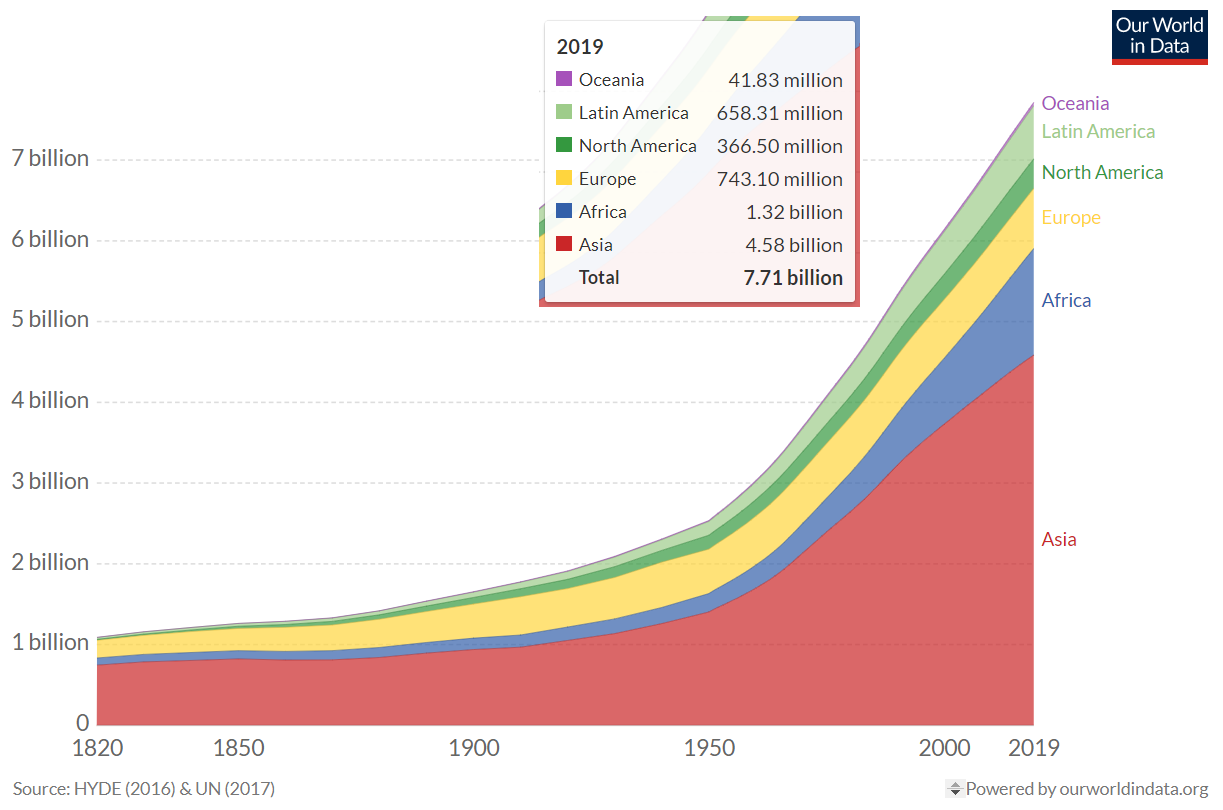
\includegraphics[width=0.7\textwidth]{Imagenes/WorldPopulationByRegion.png}
\caption{Población mundial por regiones\footnotemark}
\end{figure}
\begin{center}
7.710'000.000 de personas
\end{center}
\footnotetext[1]{\textit{World Population Growth}, Max Roser et. al., última revisión mayo 2019}
\end{frame}

\begin{frame}{Importancia del fechado de núcleos sedimentarios acuáticos}
\begin{figure}
\centering
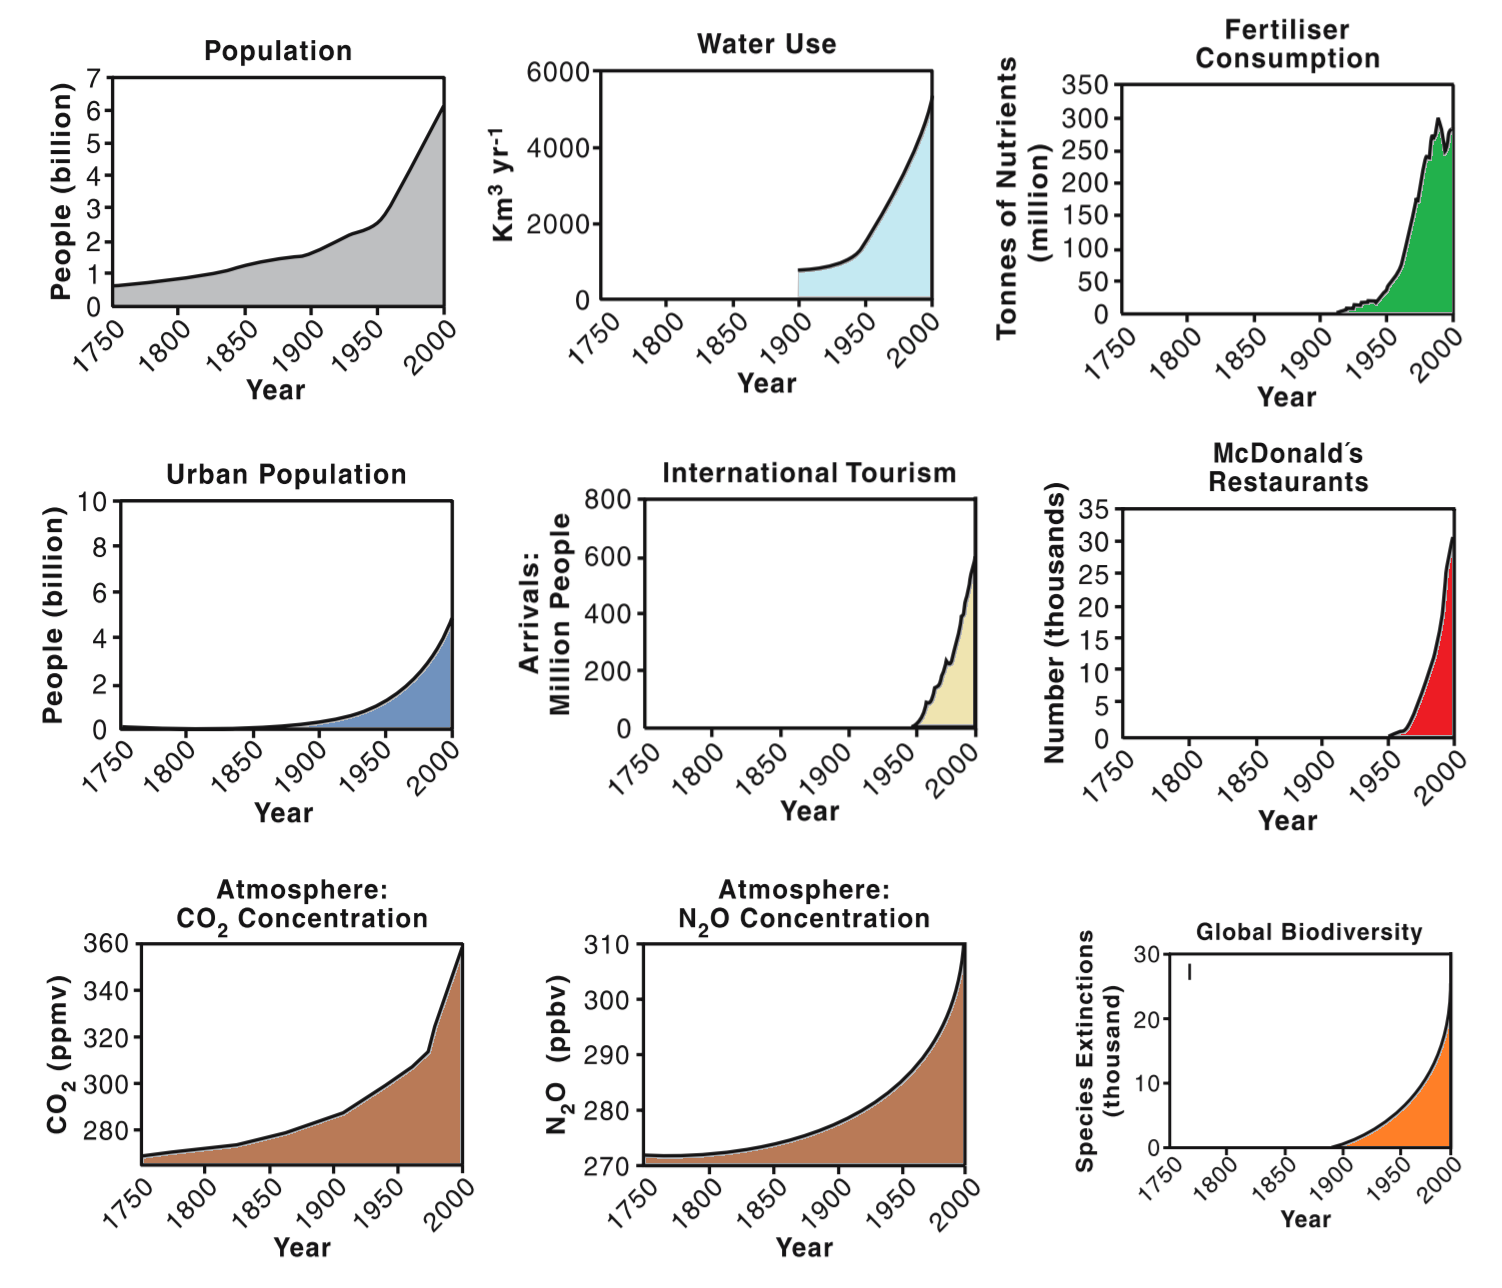
\includegraphics[width=0.55\textwidth]{Imagenes/Steffen2004.png}
\caption{Actividades humanas y cambios a escala global \footnotemark}
\end{figure}
\begin{center}
¡Cambio Global y Climático!
\end{center}
\footnotetext[1]{\textit{Global Change and the Earth System. A Planet Under Pressure}. W. Steffen et. al., 2004}
\end{frame}

\begin{frame}{Importancia del fechado de núcleos sedimentarios acuáticos}
\justifying El \textbf{Cambio Global} es el conjunto de \textit{cambios} observados de manera sistemática y a escala planetaria debido a \textbf{actividades antropogénicas}\footnotemark[1].
\\
Estos cambios quedan registrados en observatorios (\$\$\$) y archivos ambientales.
\begin{figure}
	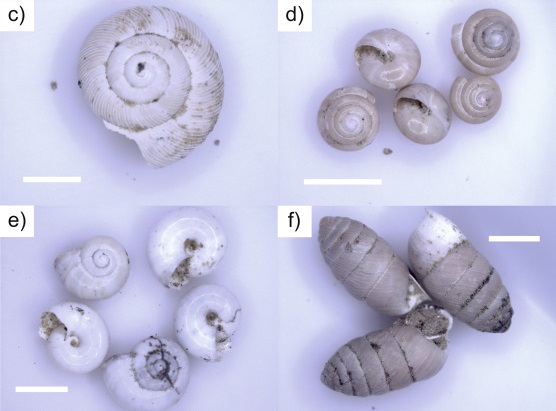
\includegraphics[height=0.35\textheight]{Imagenes/CharcoalMollusc.jpg}
	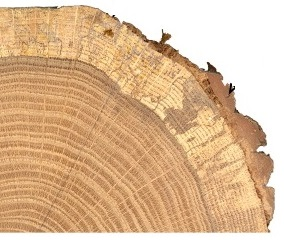
\includegraphics[height=0.35\textheight]{Imagenes/Tree.jpg}
	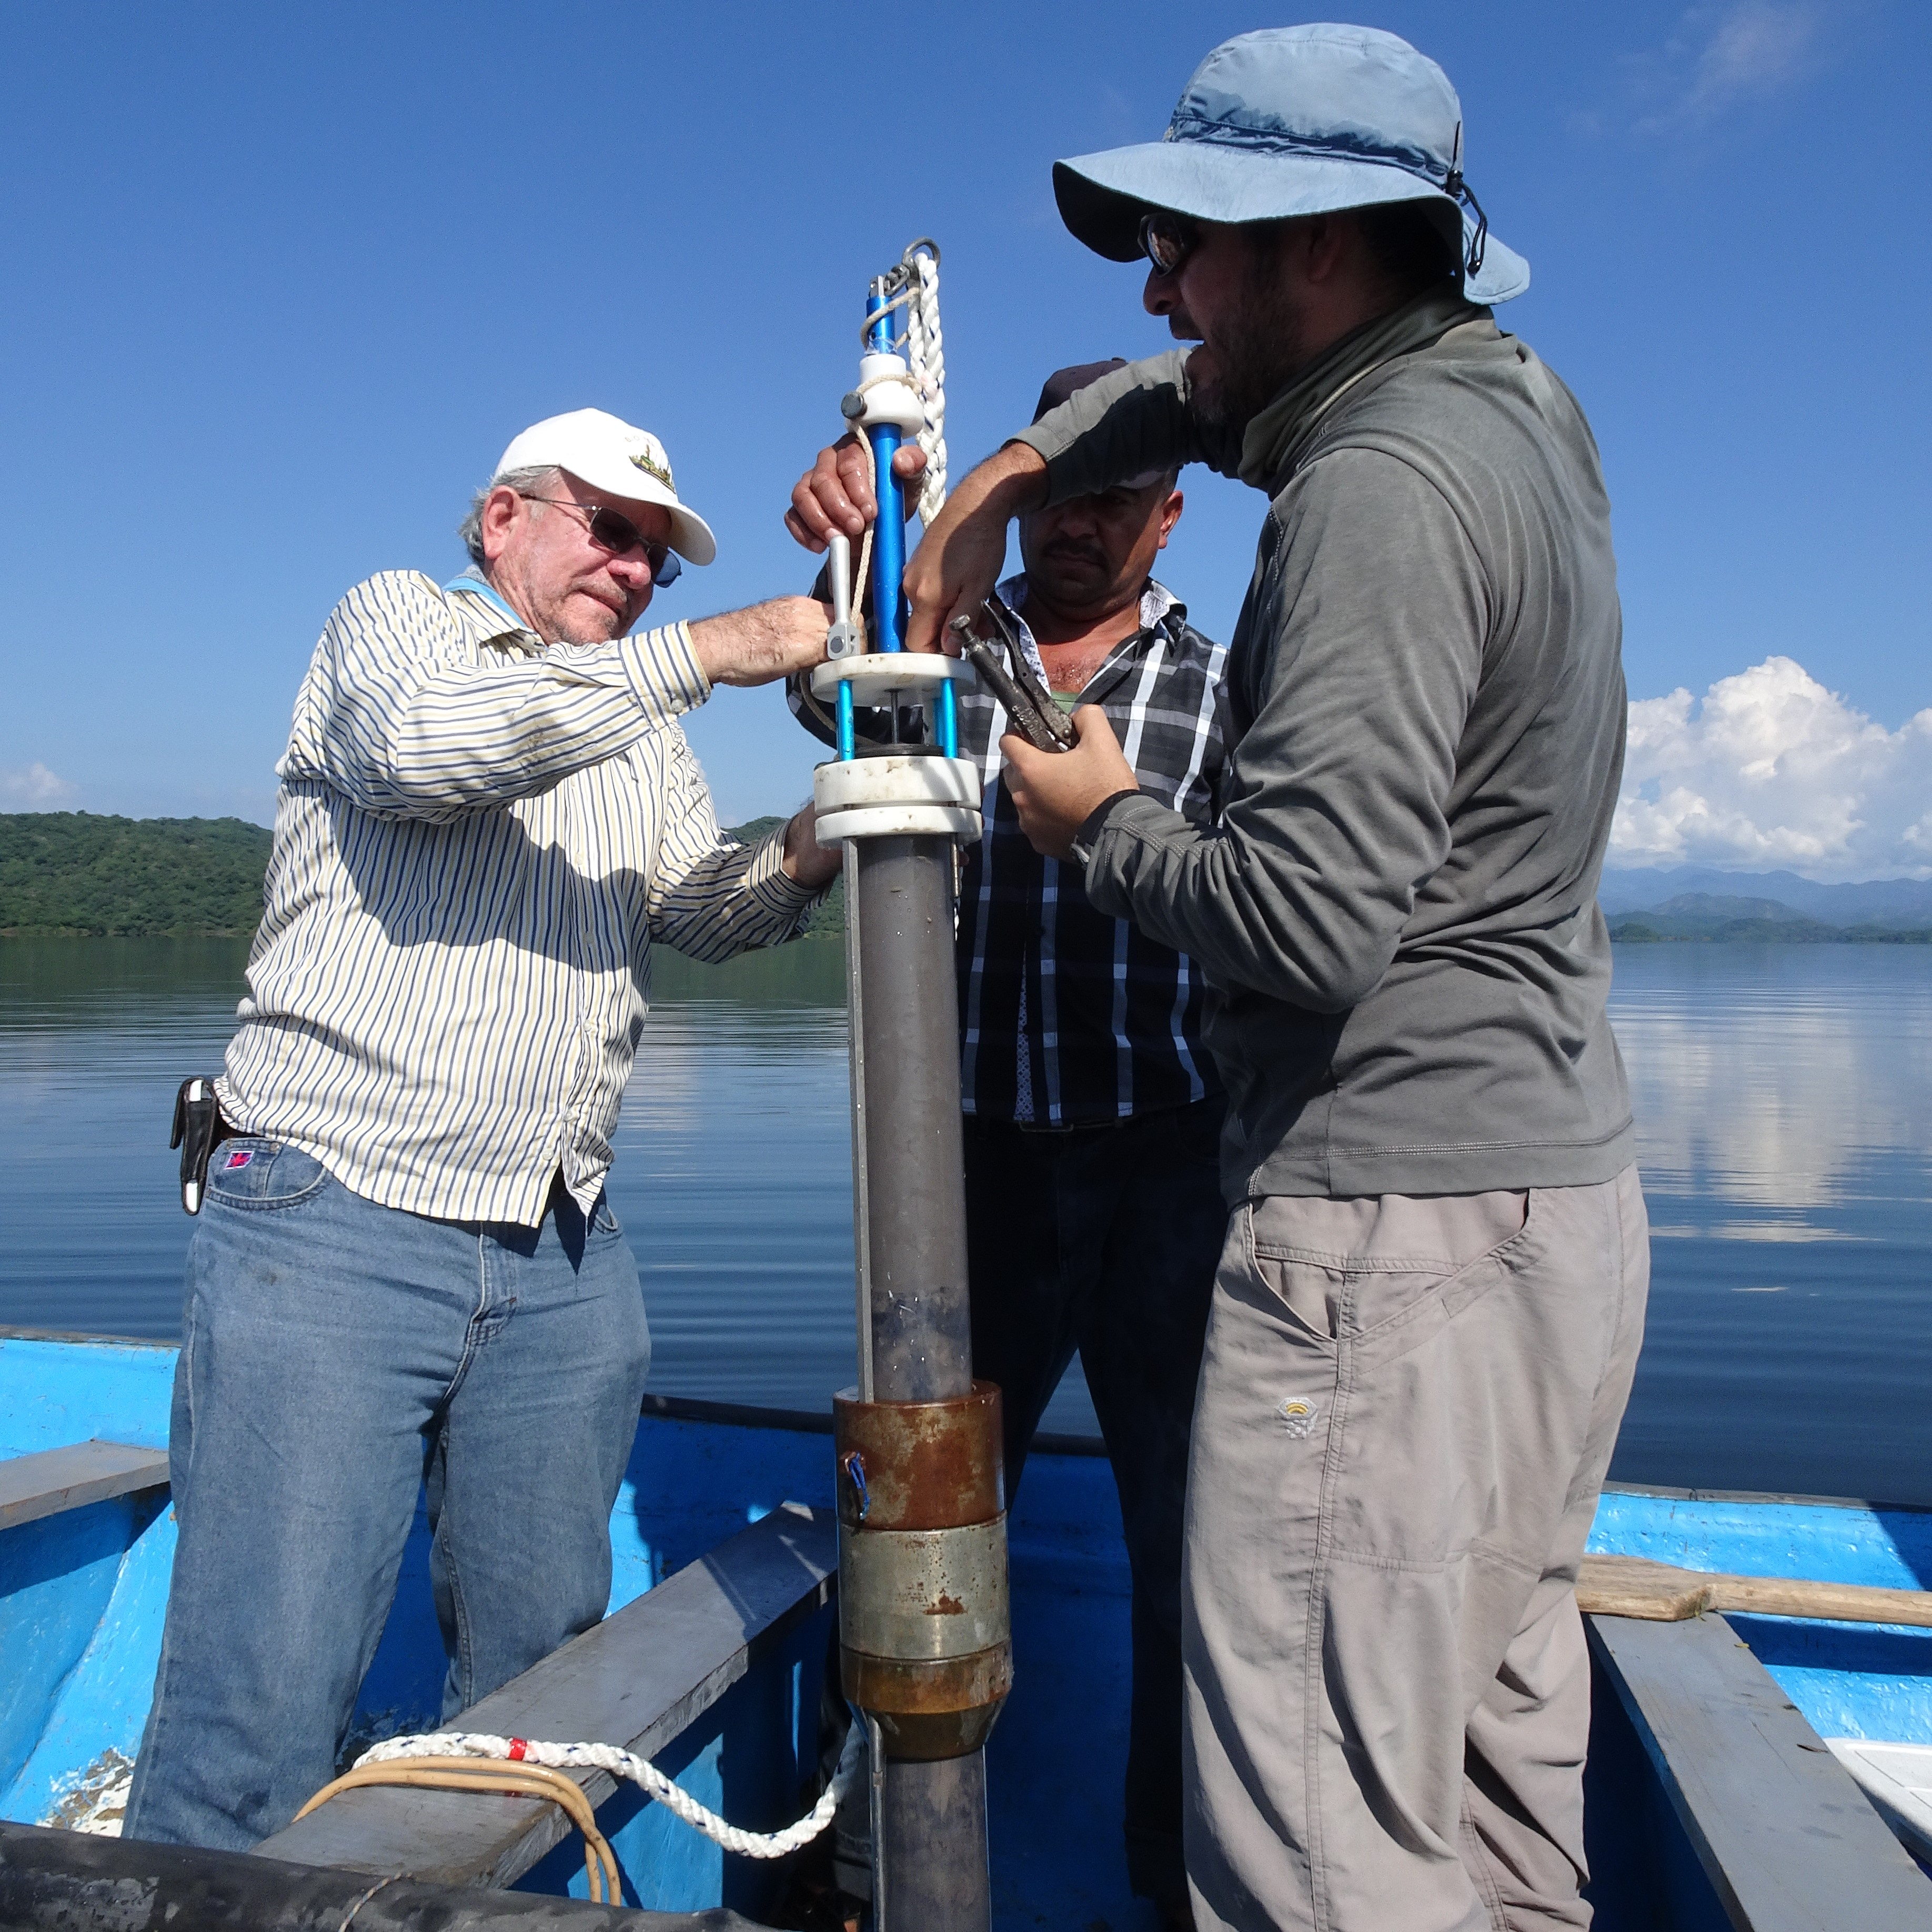
\includegraphics[height=0.35\textheight]{Imagenes/DSC01875-CUADRADA.JPG}
	\caption{Archivos ambientales: moluscos\footnotemark[2], árboles\footnotemark[3] y núcleos sedimentarios.}
	


\end{figure}
\footnotetext[1]{\textit{Beyond Global Warming: Ecology and Global Change}, Vitousek, 1994}
\footnotetext[2]{G. Újvária  Újvária et. al., Quaternary Geochronology, 2016}
\footnotetext[3]{K. Haneca et. al., Journal of Archaeological Science, 2009}

\end{frame}

\begin{frame}{Núcleos sedimentarios}
	\begin{columns}
		\begin{column}{0.47\textwidth}
			\justifying
			\begin{figure}
			\centering	
			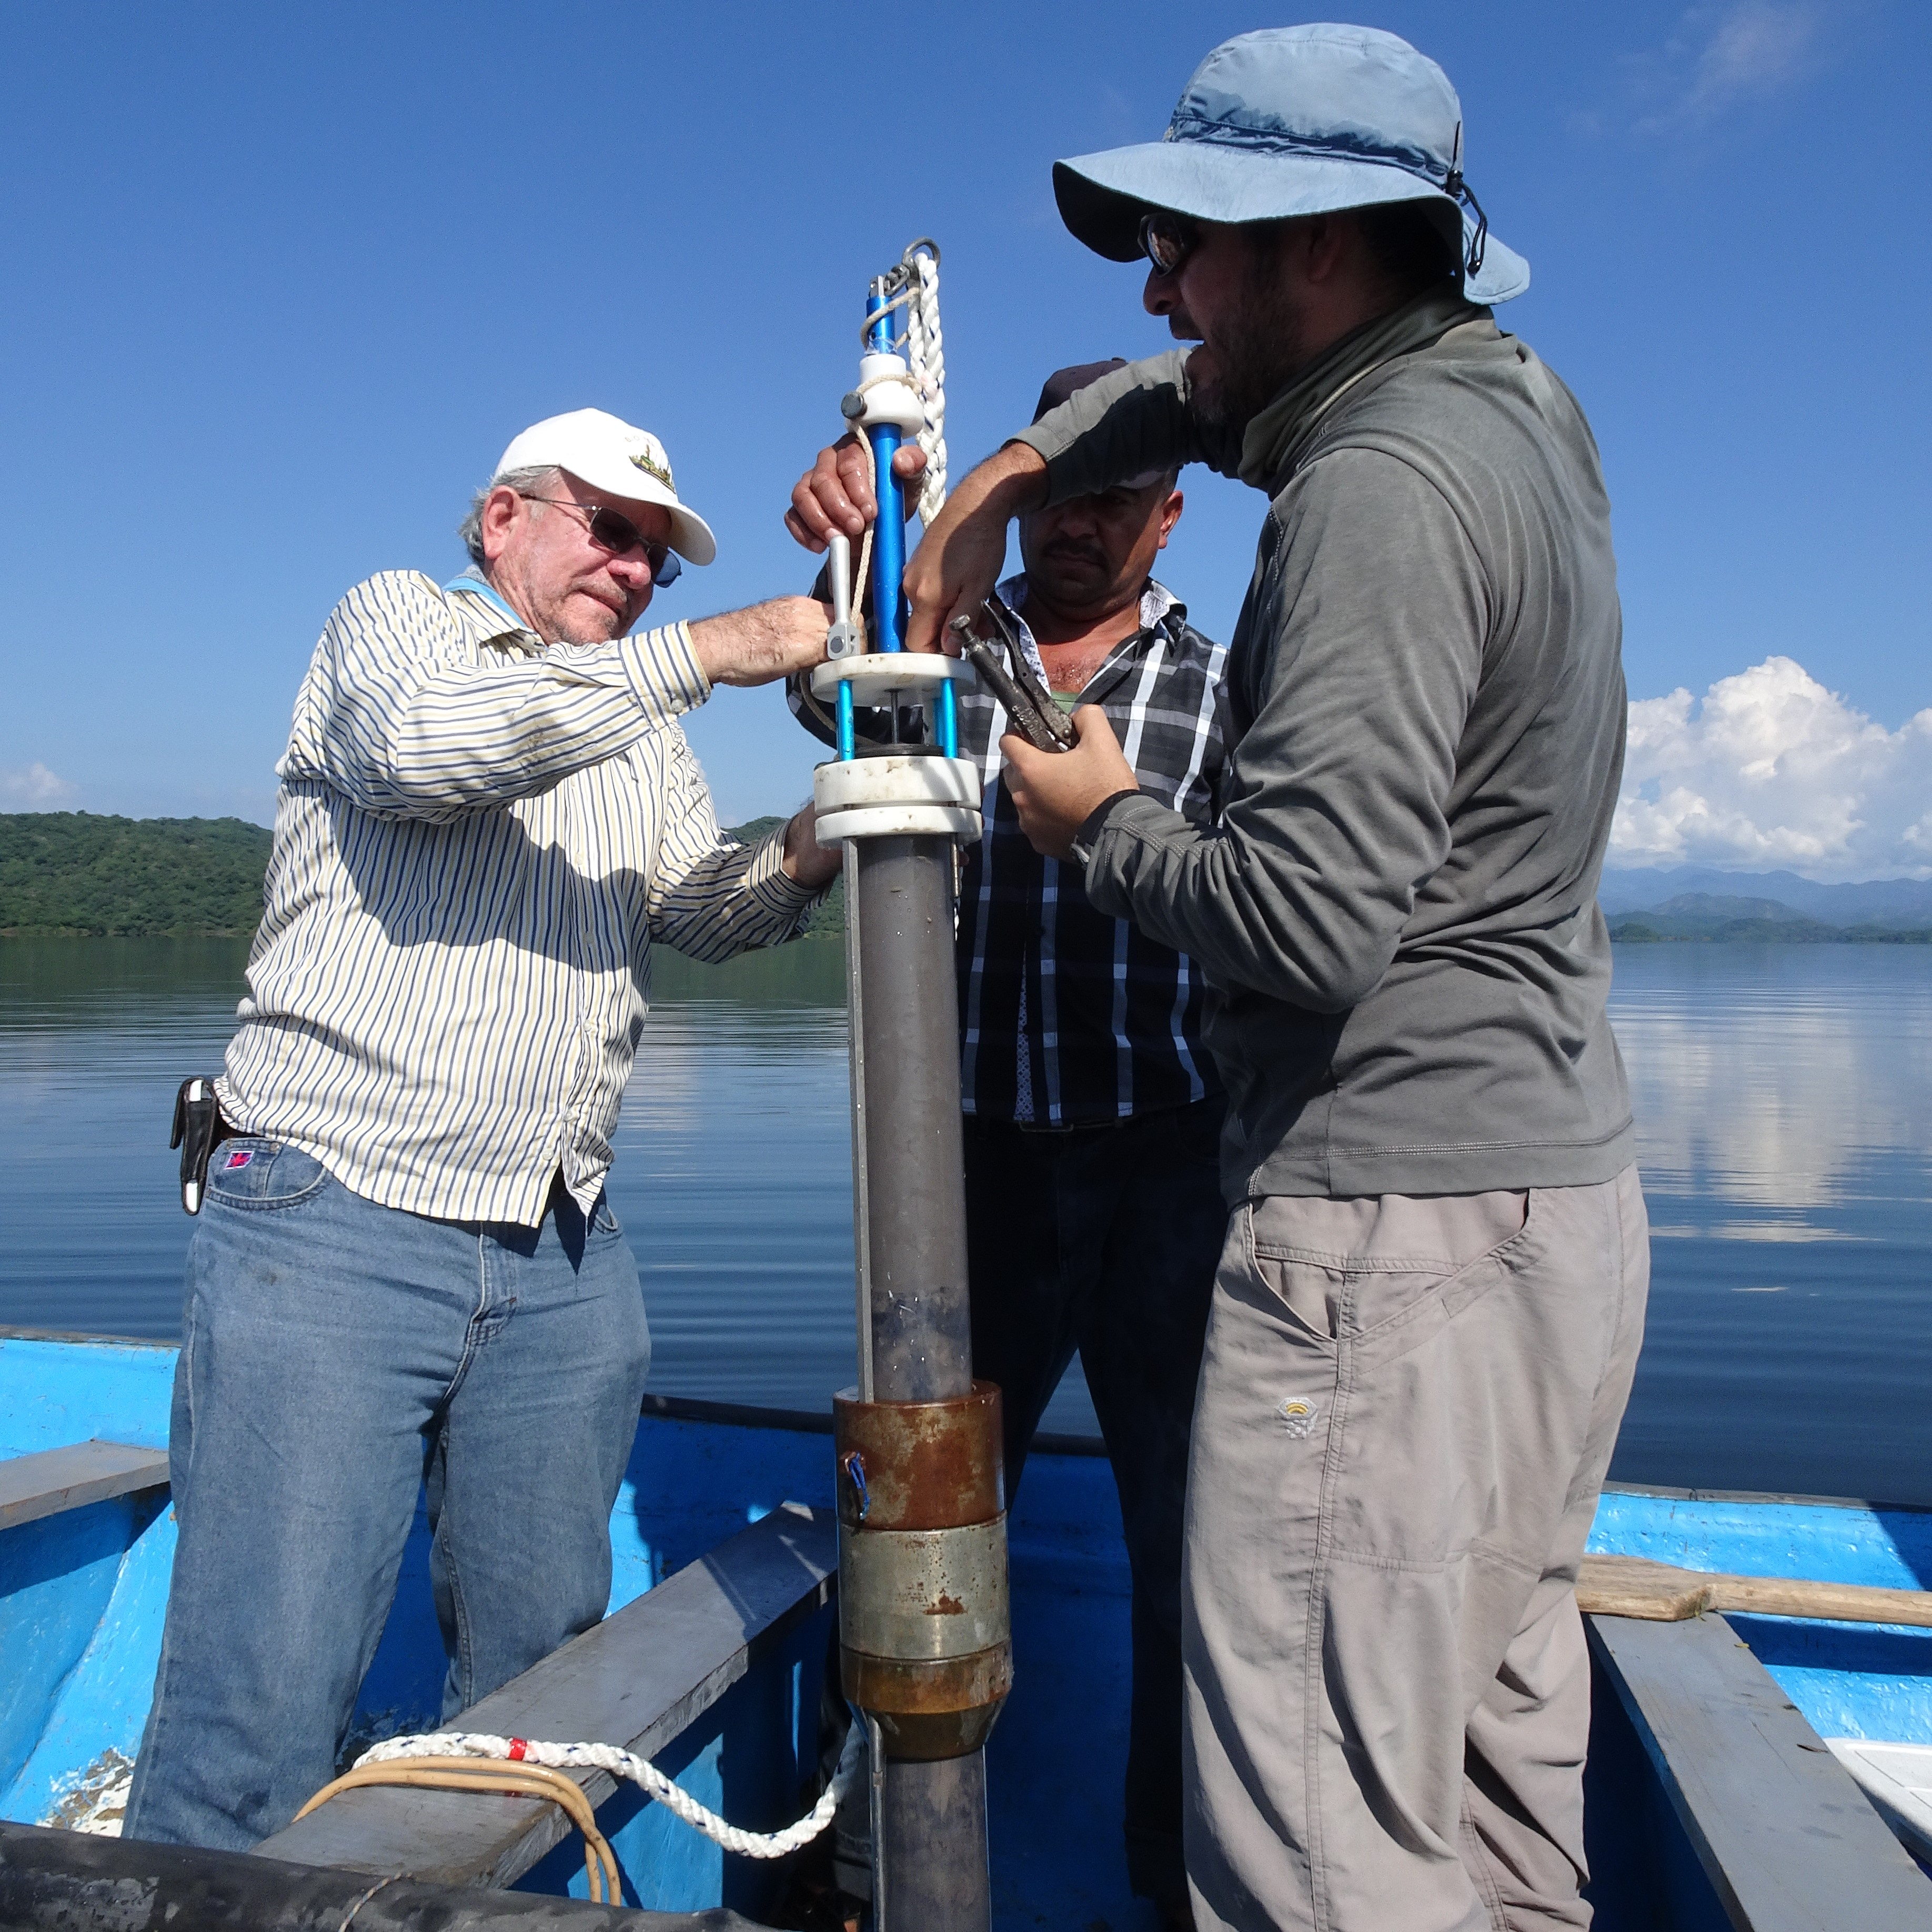
\includegraphics[height = 0.6\textheight]{Imagenes/DSC01875-CUADRADA.JPG}
			\caption{\justifying Muestreo de un núcleo sedimentario en un ambiente lacustre.}\label{Fig-MuestreoNucleoSed}
			\end{figure}
		\end{column}
		\begin{column}{0.47\textwidth}  
		\justifying Para el estudio del Cambio Global se utilizan habitualmente núcleos sedimentarios porque:
			\begin{itemize}
			\justifying
				\item son concentradores de muchas de las substancias presentes en los sistemas acuáticos (por ejemplo, la mayor parte de los contaminantes), y
				\item son relativamente fáciles de colectar y analizar. 
			\end{itemize}
			Para diagnosticar, evaluar y predecir se necesita un \textbf{marco temporal}.
		\end{column}

	\end{columns}
\end{frame}

\begin{frame}{Hipótesis y problema}
\justifying El \textbf{marco temporal} de los núcleos sedimentarios se establece con la \textbf{cantidad de \PbCero\,} presente en el sedimento.
\begin{figure}
\centering
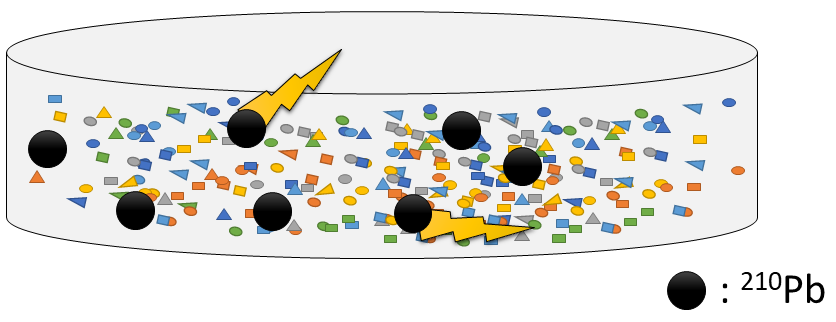
\includegraphics[width=0.7\textwidth]{Imagenes/Seccion_y_210Pb-2.png}
\end{figure}
\begin{center}
La cuantificación de \PbCero\, ($A$) depende de su composición (autoabsorción).
\\ \vspace{0.5cm}
El fechado depende de $A$, y $A$ depende de la composición.
\end{center}
\textbf{\underline{Hipótesis}:}\\
\begin{columns}
\begin{column}{0.1\textwidth}

\includegraphics[scale=0.1]{Imagenes/CaritaFeliz.jpg}
		\end{column}
		\begin{column}{0.9\textwidth}  %%<--- here
Si se conoce la composición elemental
\\
\hspace{3cm}$\rightarrow$\hspace{0.2cm} se determina mejor \PbCero
\\
\hspace{6cm}$\rightarrow$\hspace{0.2cm} fechados de mayor calidad.  
		\end{column}

	\end{columns}

\end{frame}

\begin{frame}{Hipótesis y problema}
	\begin{columns}
		\begin{column}{0.55\textwidth}
			\justifying
			El \textbf{\underline{problema}} es que la mayoría de los laboratorios que realizan el fechado con \PbCero\, \textbf{asumen una composición elemental constante}. 
			\\ \vspace{1cm}
							\begin{center}
				¿La composición \textbf{cambia} con el tiempo?
				\\ \vspace{0.4cm}
				¿Todos los mares, humedales o lagos son iguales?
			\end{center}
		\end{column}
		\begin{column}{0.4\textwidth}  %%<--- here
			\begin{figure}
				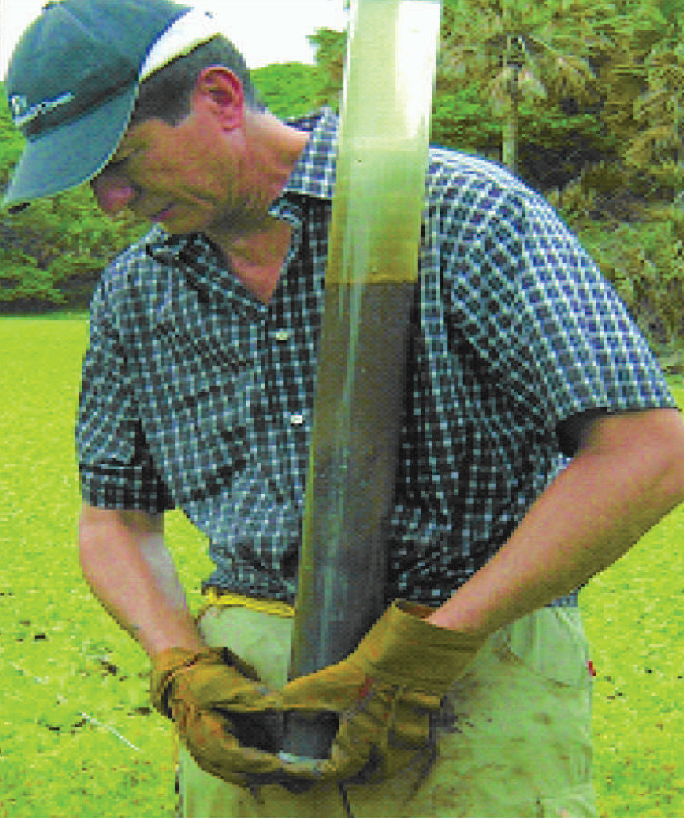
\includegraphics[width=0.8\textwidth]{Imagenes/RecoleccionCore.png}
				\caption{\justifying Recolección manual de un núcleo sedimentario\footnotemark[4] }
			\end{figure}
		\end{column}
	\footnotetext[4]{\textit{Radiocronología de sedimentos costeros utilizando \PbCero: modelos, validación y aplicaciones}, Sanchez-Cabeza et. al., 2012.}
	\end{columns}


\end{frame}

\begin{frame}{Objetivo general}
	\begin{columns}
		\begin{column}{0.47\textwidth}
			\justifying

		\end{column}
		\begin{column}{0.47\textwidth}  
			\justifying
			
\includegraphics[scale=0.2]{Imagenes/Objetivo.jpg}
			\\
			El objetivo general es \textbf{mejorar la cuantificación} de los radionúclidos utilizados en el fechado de sedimentos recientes (\textbf{\PbCero\, y \PbCuatro}) a través de \textbf{correcciones de densidad y composición}.
			\\ \vspace{0.5cm}
			El objetivo no es realizar la calibración de un sistema de espectrometría gamma ni fechar núcleos sedimentarios.
		\end{column}
	\end{columns}
\end{frame}

\section{Introducción y metodología}

\begin{frame}{Actividad de un núcleo radiactivo}
	\begin{columns}
			\begin{column}{0.68\textwidth}
			\justifying
			La actividad $A$ de un radionúclido es el número de desintegraciones nucleares por unidad de tiempo $t$ y es proporcional a la cantidad de átomos radiactivos $N$ presentes en la muestra
			\begin{equation}
			A = - \dfrac{\text{d}N}{\text{d}t} = \lambda\, N, \hspace{0.5cm} \lambda = \frac{\ln(2)}{T_{\frac{1}{2}}},
			\end{equation}
			donde $T_{\frac{1}{2}}$ es el tiempo en el cual la actividad de un radionúclido decrece a la mitad de su valor original. 
\begin{figure}
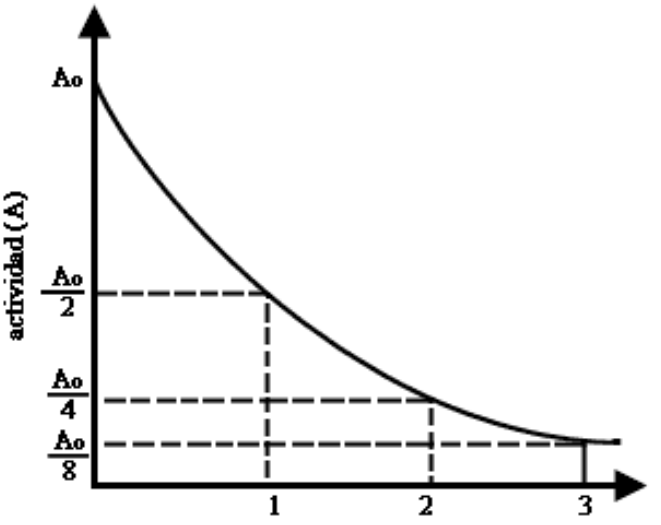
\includegraphics[width=0.4\textwidth]{Imagenes/ExponentialDecay.png}
\caption{\justifying Comportamiento exponencial del decaimiento radiactivo.}
\end{figure}			
			
		\end{column}
		\begin{column}{0.3\textwidth}  
			\justifying
			\begin{figure}
			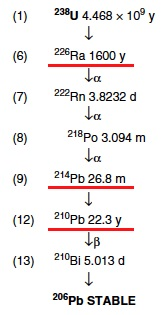
\includegraphics[width=0.7\textwidth]{Imagenes/UDacay-2.jpg}
			\caption{\justifying Serie de desintegración de \UDosTresOcho\footnotemark[1].  \textbf{¡\hyperlink{EquilibrioSecular}{\beamerbutton{Equilibrio Secular}}!}}
			\end{figure}
		\end{column}
	\end{columns}
\footnotetext[1]{Gilmore, G., \textit{Practical gamma-ray spectrometry}, Wiley, 2008.}
\end{frame}

\begin{frame}{\PbCero\, y \PbCuatro}
	\begin{columns}

			\begin{column}{0.5\textwidth}
			\begin{figure}
		\centering
		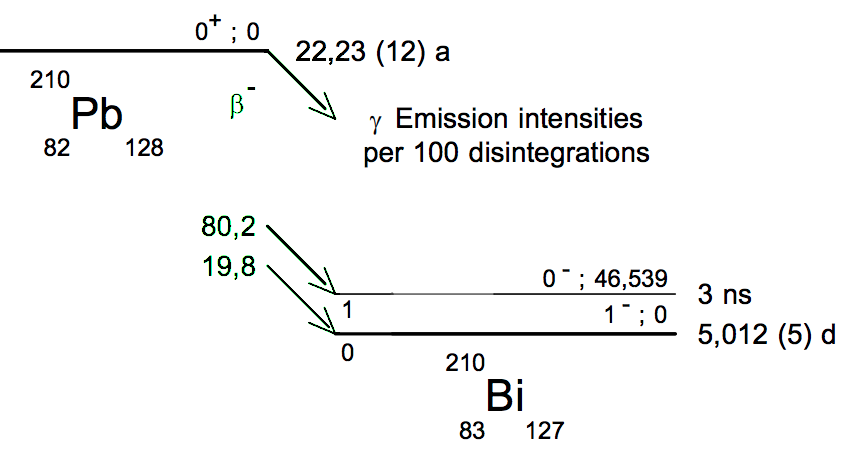
\includegraphics[width=1\textwidth]{Imagenes/210Pb-Paint.png}
		\caption{\justifying Esquema de desintegración de \PbCero\footnotemark[1].}
	\end{figure}
		\end{column}
		\begin{column}{0.5\textwidth}  
			\begin{figure}
		\centering
		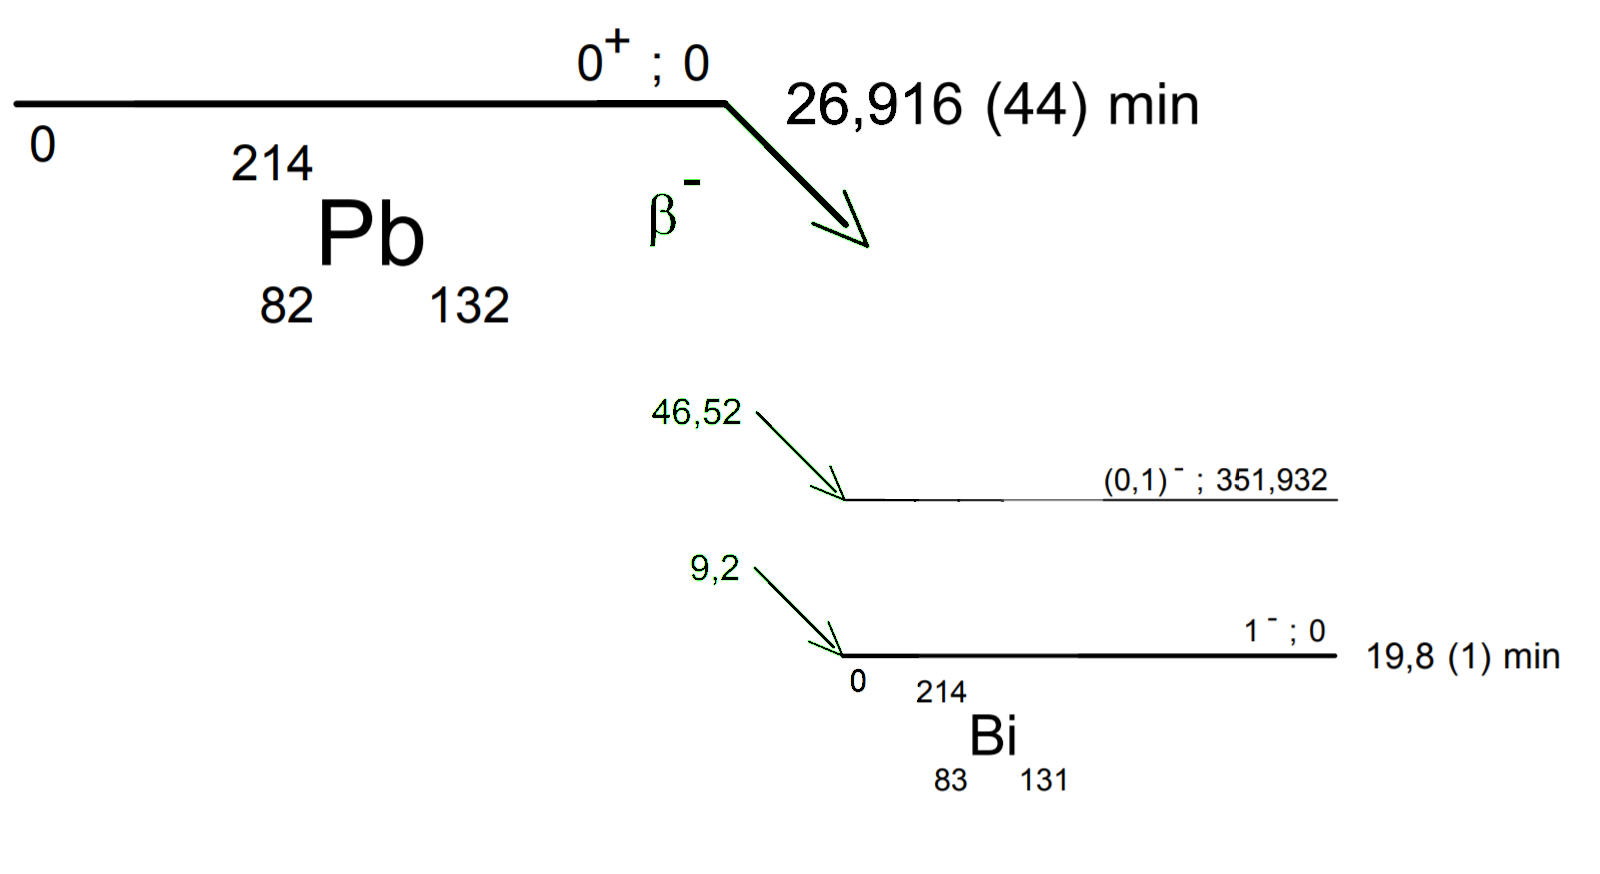
\includegraphics[width=1\textwidth]{Imagenes/214Pb-Paint.png}
		\caption{\justifying Esquema de desintegración de \PbCuatro\footnotemark[1].}
	\end{figure}
		\end{column}
	\end{columns}
	\begin{equation}
		T_{\frac{1}{2}}(^{210}\text{Pb}) = 22.23(12) \text{ años,} \hspace{1cm } T_{\frac{1}{2}}(^{214}\text{Pb}) = 26.916(44) \text{ minutos.} 
	\end{equation}
		\begin{equation}
		E(^{210}\text{Pb}) = 46.534 \text{ keV,} \hspace{1cm } E(^{214}\text{Pb}) = 351.932 \text{ keV.} 
	\end{equation}
\footnotetext[1]{Data Decay Evaluation Project, \url{http://www.nucleide.org/DDEP_WG/DDEPdata.htm}}
\end{frame}

\begin{frame}{Ciclo de \PbCero\, en ecosistemas acuáticos}
	\begin{columns}
		\begin{column}{0.7 \textwidth}
			\justifying
			\begin{figure}
				\centering
				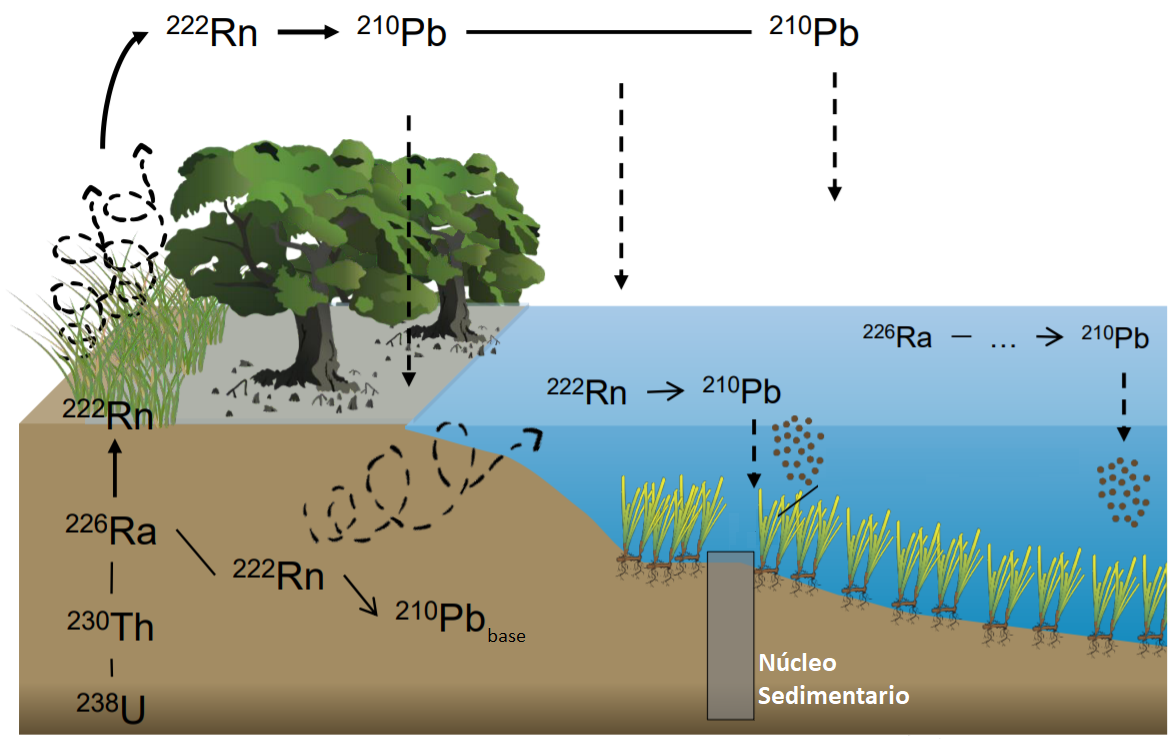
\includegraphics[width=0.99\textwidth]{Imagenes/Ciclo210PbAcuatico.png}
				\caption{\hyperlink{Ciclo}{\beamerbutton{Ciclo}} de \PbCero\, en un sistema costero\footnotemark[1].}\label{Fig-Ciclo210Pb}
			\end{figure}
			\begin{equation}
						^{210}\text{Pb}_\text{total} =  ^{210}\text{Pb}_\text{base} + ^{210}\text{Pb}_\text{ex} 
			\end{equation}

		\end{column}
		\begin{column}{0.27\textwidth}  
			\justifying
			\PbCeroEx\, es \PbCero\, generado en la atmósfera y en los cuerpos de agua.
			\begin{figure}
		\centering
		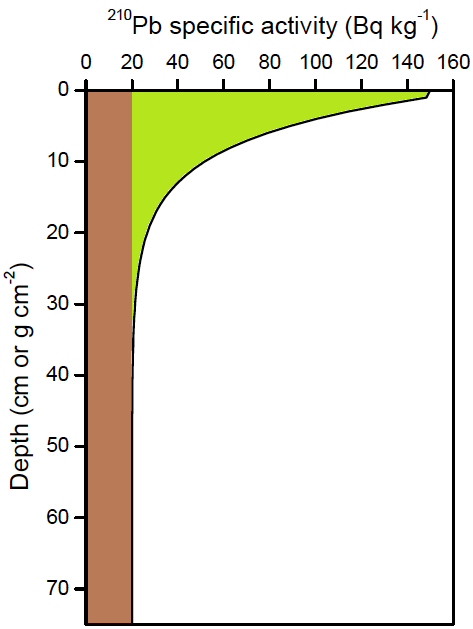
\includegraphics[width=\textwidth]{Imagenes/PerfilIdeal-2.png}
		\caption{\justifying Perfil ideal de actividad específica de \PbCero\footnotemark[1].}
	\end{figure}			
			
		\end{column}
	\end{columns}
\footnotetext[1]{Arias-Ortiz et al., Biogeosciences, 15(22):6791–6818, 2018}
\end{frame}

\begin{frame}{Fechado de núcleos sedimentarios}
\begin{center}
El \hyperlink{Fechado}{\beamerbutton{modelo}} utilizado asume que el flujo de \PbCero\, es constante.
 \end{center}

\begin{columns}
		\begin{column}{0.4\textwidth}
			\justifying
\begin{figure}
 \centering
 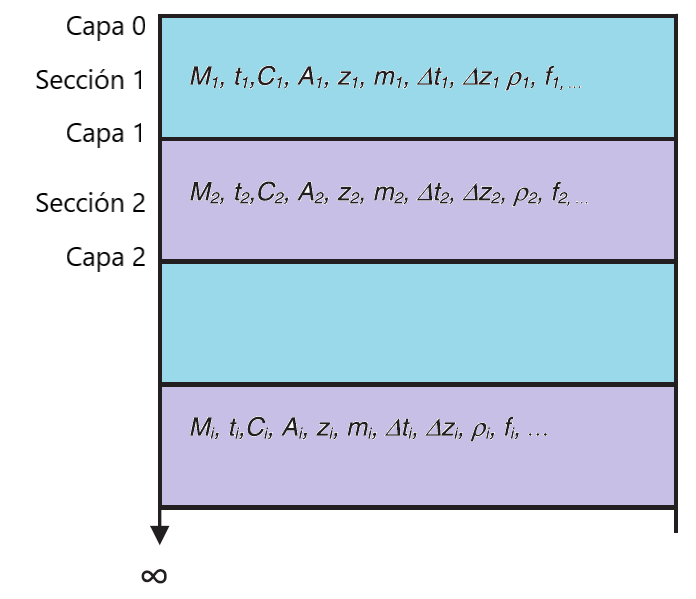
\includegraphics[width=\textwidth]{Imagenes/EsquemaNucleoSed-4.png}
 \caption{Sección y capas de corte para el fechado de un núcleo sedimentario\footnotemark[1].}
\end{figure}
		\end{column}
		\begin{column}{0.5\textwidth}  
			\justifying
			Sea 
			\begin{itemize}
			\item $A_i$: Actividad específica de \PbCeroEx\, de la sección $i$-ésima, 
			\item $m_i$: profundidad másica promedio de la sección $i$-ésima.
			\end{itemize}						
			Entonces el fechado de la capa $i$-ésima es
			\begin{equation}
t(i) = \dfrac{1}{\lambda}\,\ln\left(\dfrac{\sum_{j=1}^\infty A_j\, m_j}{ \sum_{j=i+1}^\infty A_j\, m_j}\right). 
			\end{equation}			

		\end{column}
	\end{columns}
\footnotetext[1]{Sanchez-Cabeza y Ruiz-Fernández, Geochimica et Cosmochimica Acta, 82:183–200, 2012.}
\end{frame}

\begin{frame}{Interacción de la radiación con la materia}
\justifying Los canales de interacción entre los rayos gamma y la materia \textbf{dependen de la energía de la radiación incidente}.
	\begin{columns}
		\begin{column}{0.49\textwidth}
		\begin{center}
		\textbf{Efecto fotoeléctrico}
		\begin{figure}
		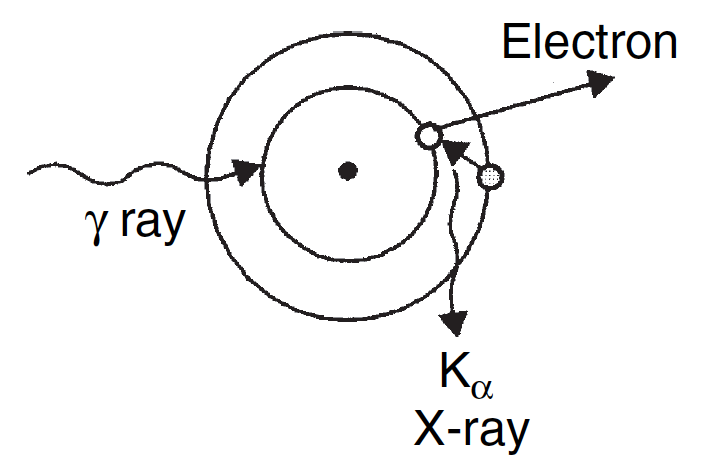
\includegraphics[height = 0.3\textheight]{Imagenes/Photoelectric-2.png}
		\caption{\justifying Mecanismo del efecto fotoeléctrico\footnotemark[1].}
		\end{figure}
		\end{center}			
		\end{column}
		\begin{column}{0.49\textwidth}  
		\begin{center}
		\textbf{Efecto Compton}
		\begin{figure}
		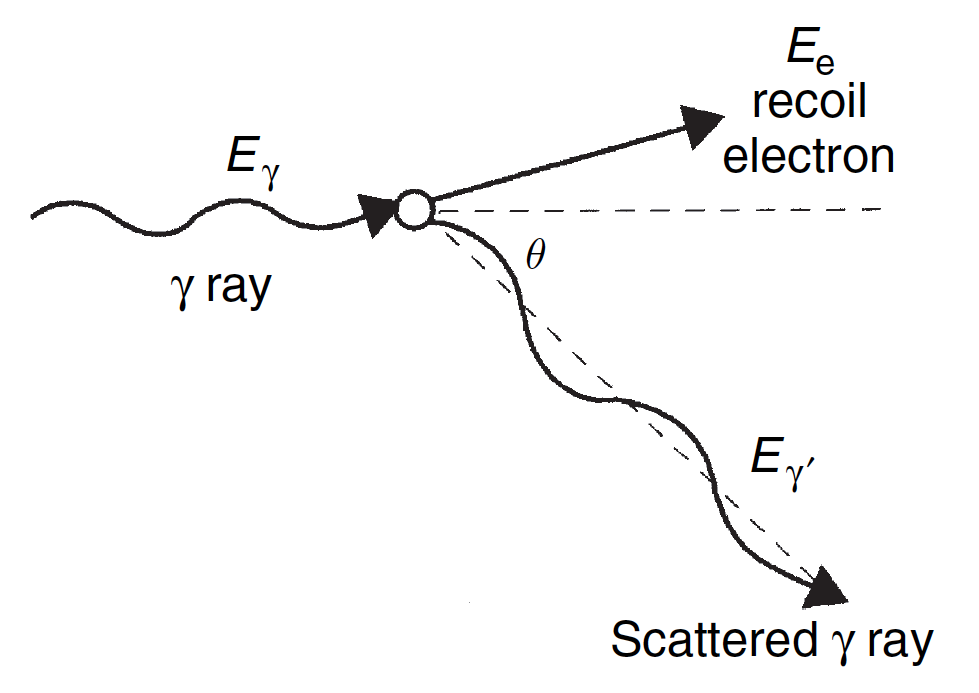
\includegraphics[height = 0.3\textheight]{Imagenes/Compton.png}
		\caption{\justifying Mecanismo del efecto Compton\footnotemark[1].}
		\end{figure}
		\end{center}
		\end{column}
	\end{columns}
Para $E >1.022$ MeV, existe la probabilidad del proceso \textbf{Formación de Pares}.
	
\footnotetext[1]{Gilmore, G., \textit{Practical gamma-ray spectrometry}, Wiley, 2008.}
\end{frame}

\begin{frame}{Sección eficaz total}
	\begin{columns}
		\begin{column}{0.65\textwidth}
		\begin{figure}
			\centering
			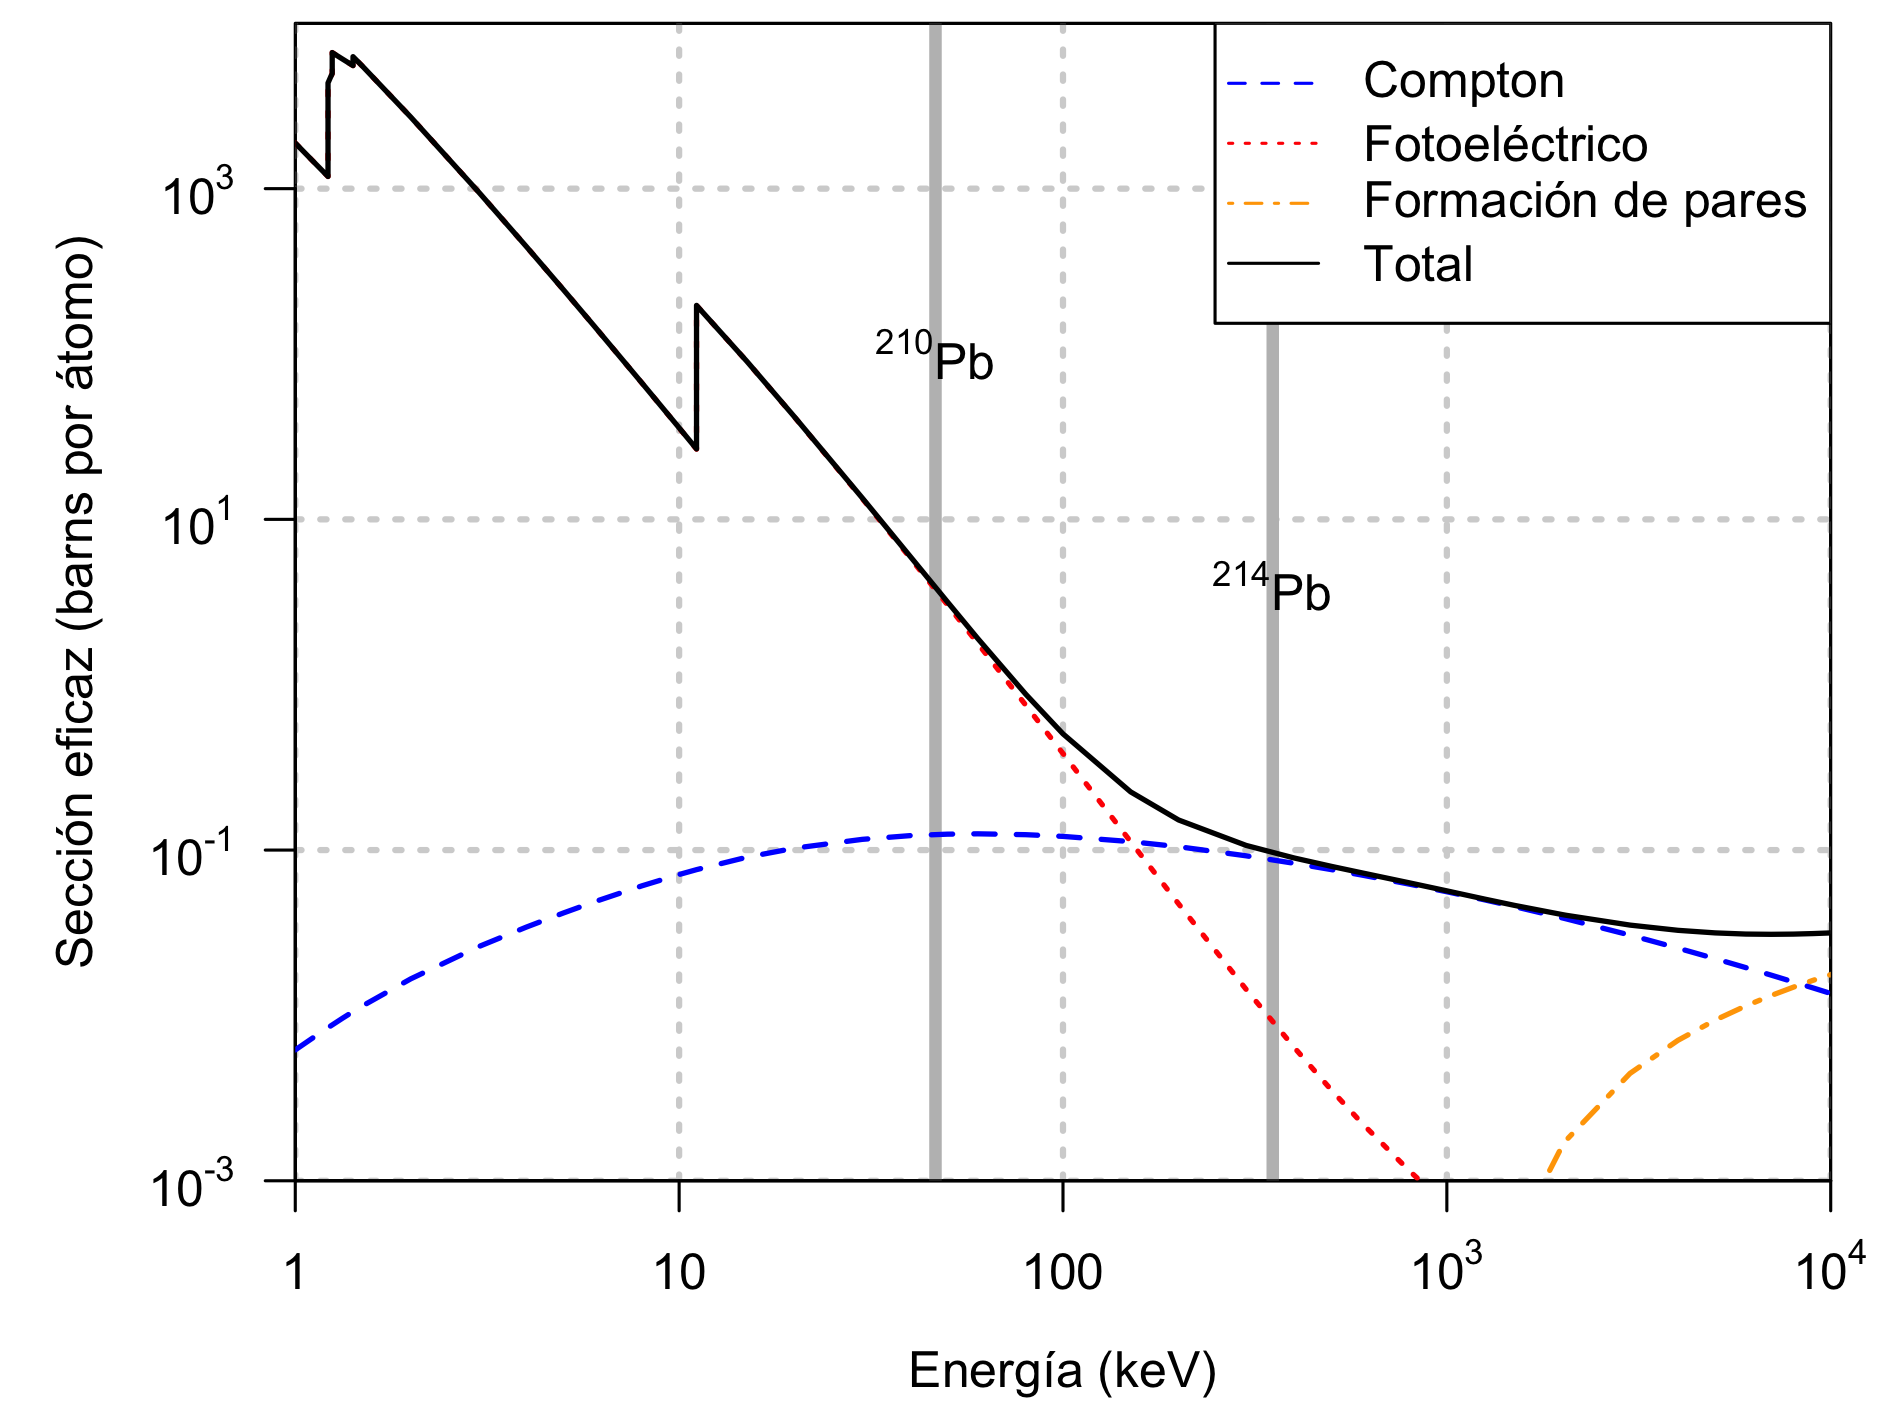
\includegraphics[width=1\textwidth]{Imagenes/CrossSectionGe.png}
			\caption{\justifying \hyperlink{SeccionEficaz}{\beamerbutton{Sección eficaz}} total y parcial (fotoeléctrico, Compton y Formación de pares) de fotones sobre germanio.}
		\end{figure}
		\end{column}
		\begin{column}{0.3\textwidth}  
		\justifying
		La sección eficaz total $\sigma_\text{total}$ es
		\begin{equation}
			\sigma_\text{total} = \sum_i \sigma_i.
		\end{equation}
		La interacción de la radiación con la materia se cuantifica a través del \hyperlink{Masico}{\beamerbutton{coeficiente}} \textbf{másico de atenuación}  $\dfrac{\mu}{\rho}$ 
\\ \vspace{1cm}
¡Incluye la densidad! 
		\end{column}
	\end{columns}
\end{frame}

\begin{frame}{Detectores de germanio hiper puro en configuración de pozo}
	\begin{columns}
		\begin{column}{0.68\textwidth}  
\begin{figure}
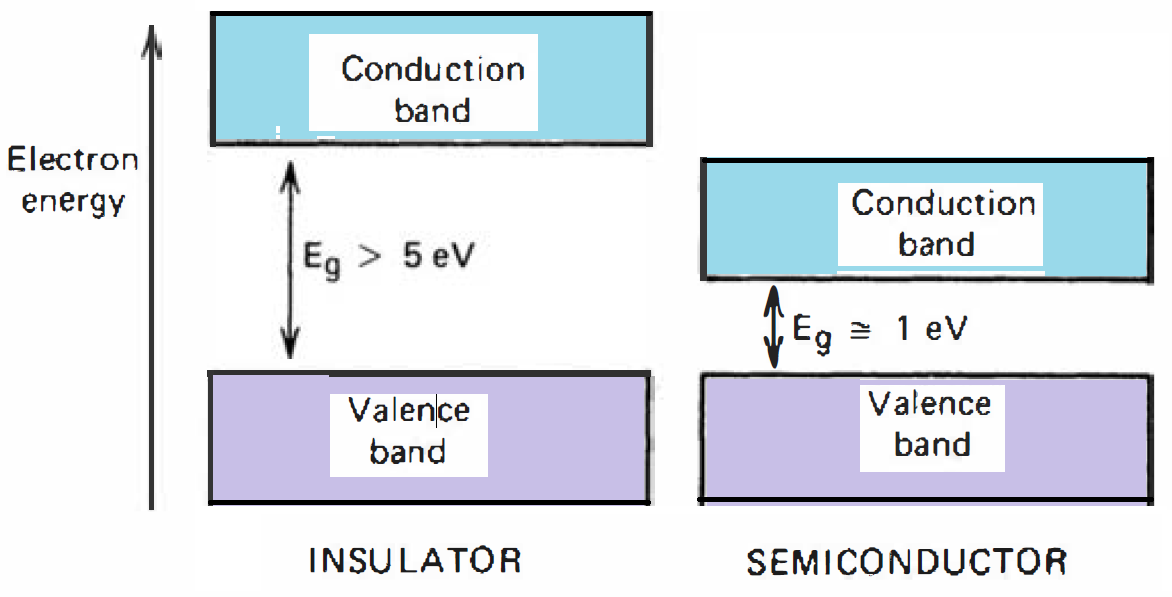
\includegraphics[width=0.5\textwidth]{Imagenes/SemiConductor.png}
\caption{Estructura de bandas para las energías electrónicas en aislantes y semiconductores\footnotemark[1].}
\end{figure}
			\begin{itemize}
			\justifying		
\item Densidad elevada en comparación con detectores gaseosos. 
\item Los detectores de Ge son ampliamente utilizados en física nuclear y necesitan refrigeración debido a su banda de energía prohibida tan pequeña (0.66 eV). 
\item[*] Proporcionan un ángulo sólido cercano a $4\,\pi$.
\item[*] La eficiencia adquiere su valor máximo en la parte inferior del pozo.
			\end{itemize}
		\end{column}
		\begin{column}{0.28\textwidth}
			\begin{figure}
			\centering
			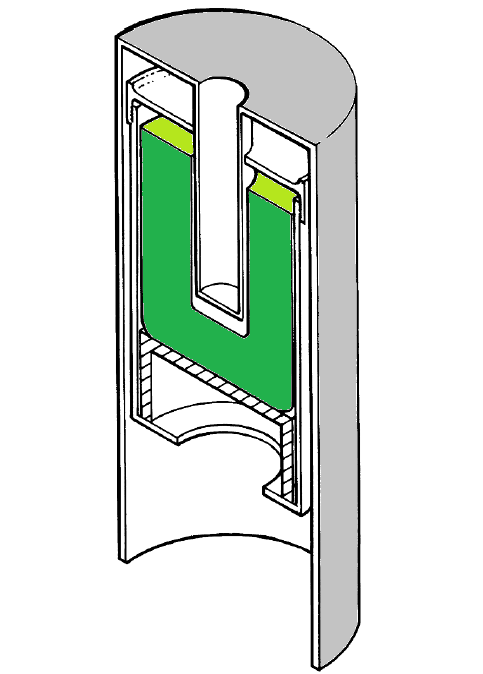
\includegraphics[width=1\textwidth]{Imagenes/WellDetectorSimply-2.png}
			\caption{\justifying Vista isométrica simplificada de un detector de Ge en configuración de pozo\footnotemark[2]}
			\end{figure}
		\end{column}
	\end{columns}
	\footnotetext[1]{\textit{Radiation Detection and Measurement}, G. F. Knoll, 2010.}
	\footnotetext[2]{ORTEC, GWL Series Coaxial HPGe Detector Product Configuration Guide, 2006.}
\end{frame}

\begin{frame}{Sistema de espectrometría gamma}
	\begin{columns}
		\begin{column}{0.45\textwidth}
			\begin{figure}
			\centering
			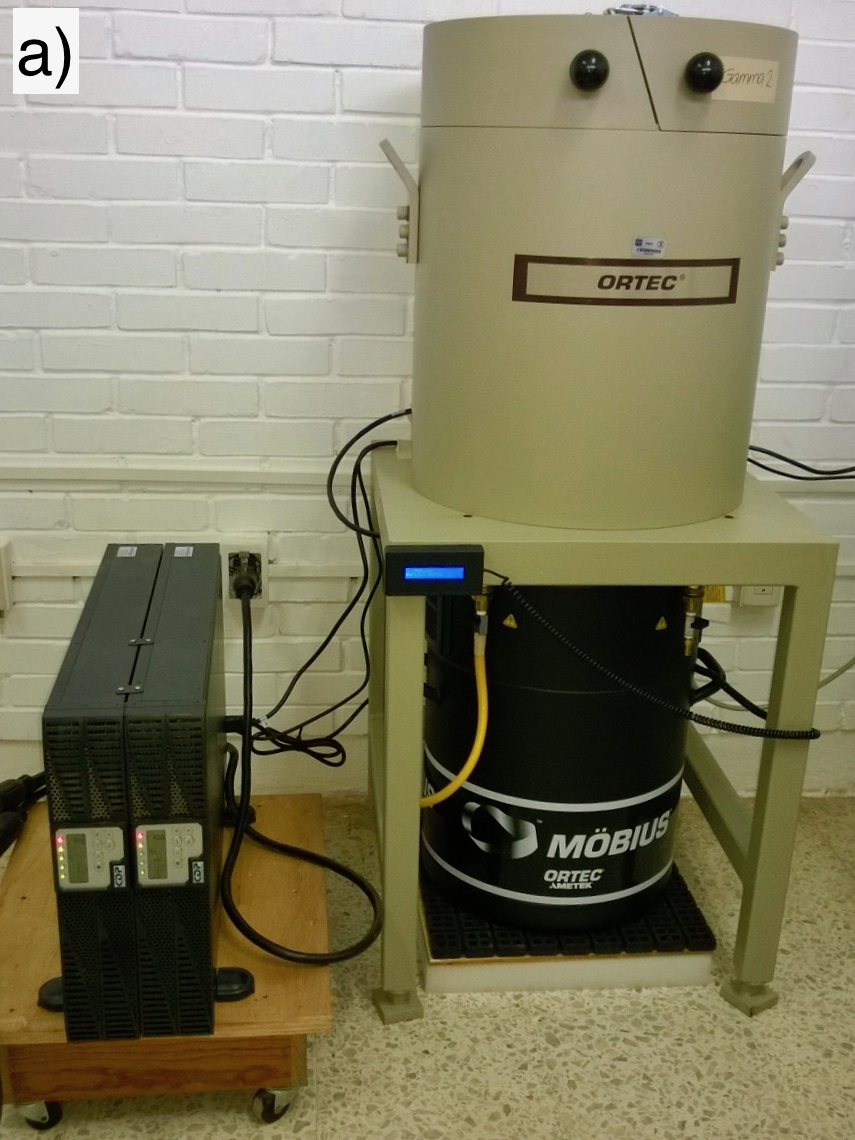
\includegraphics[height=0.45\textheight]{Imagenes/GammaSystem.jpg}
			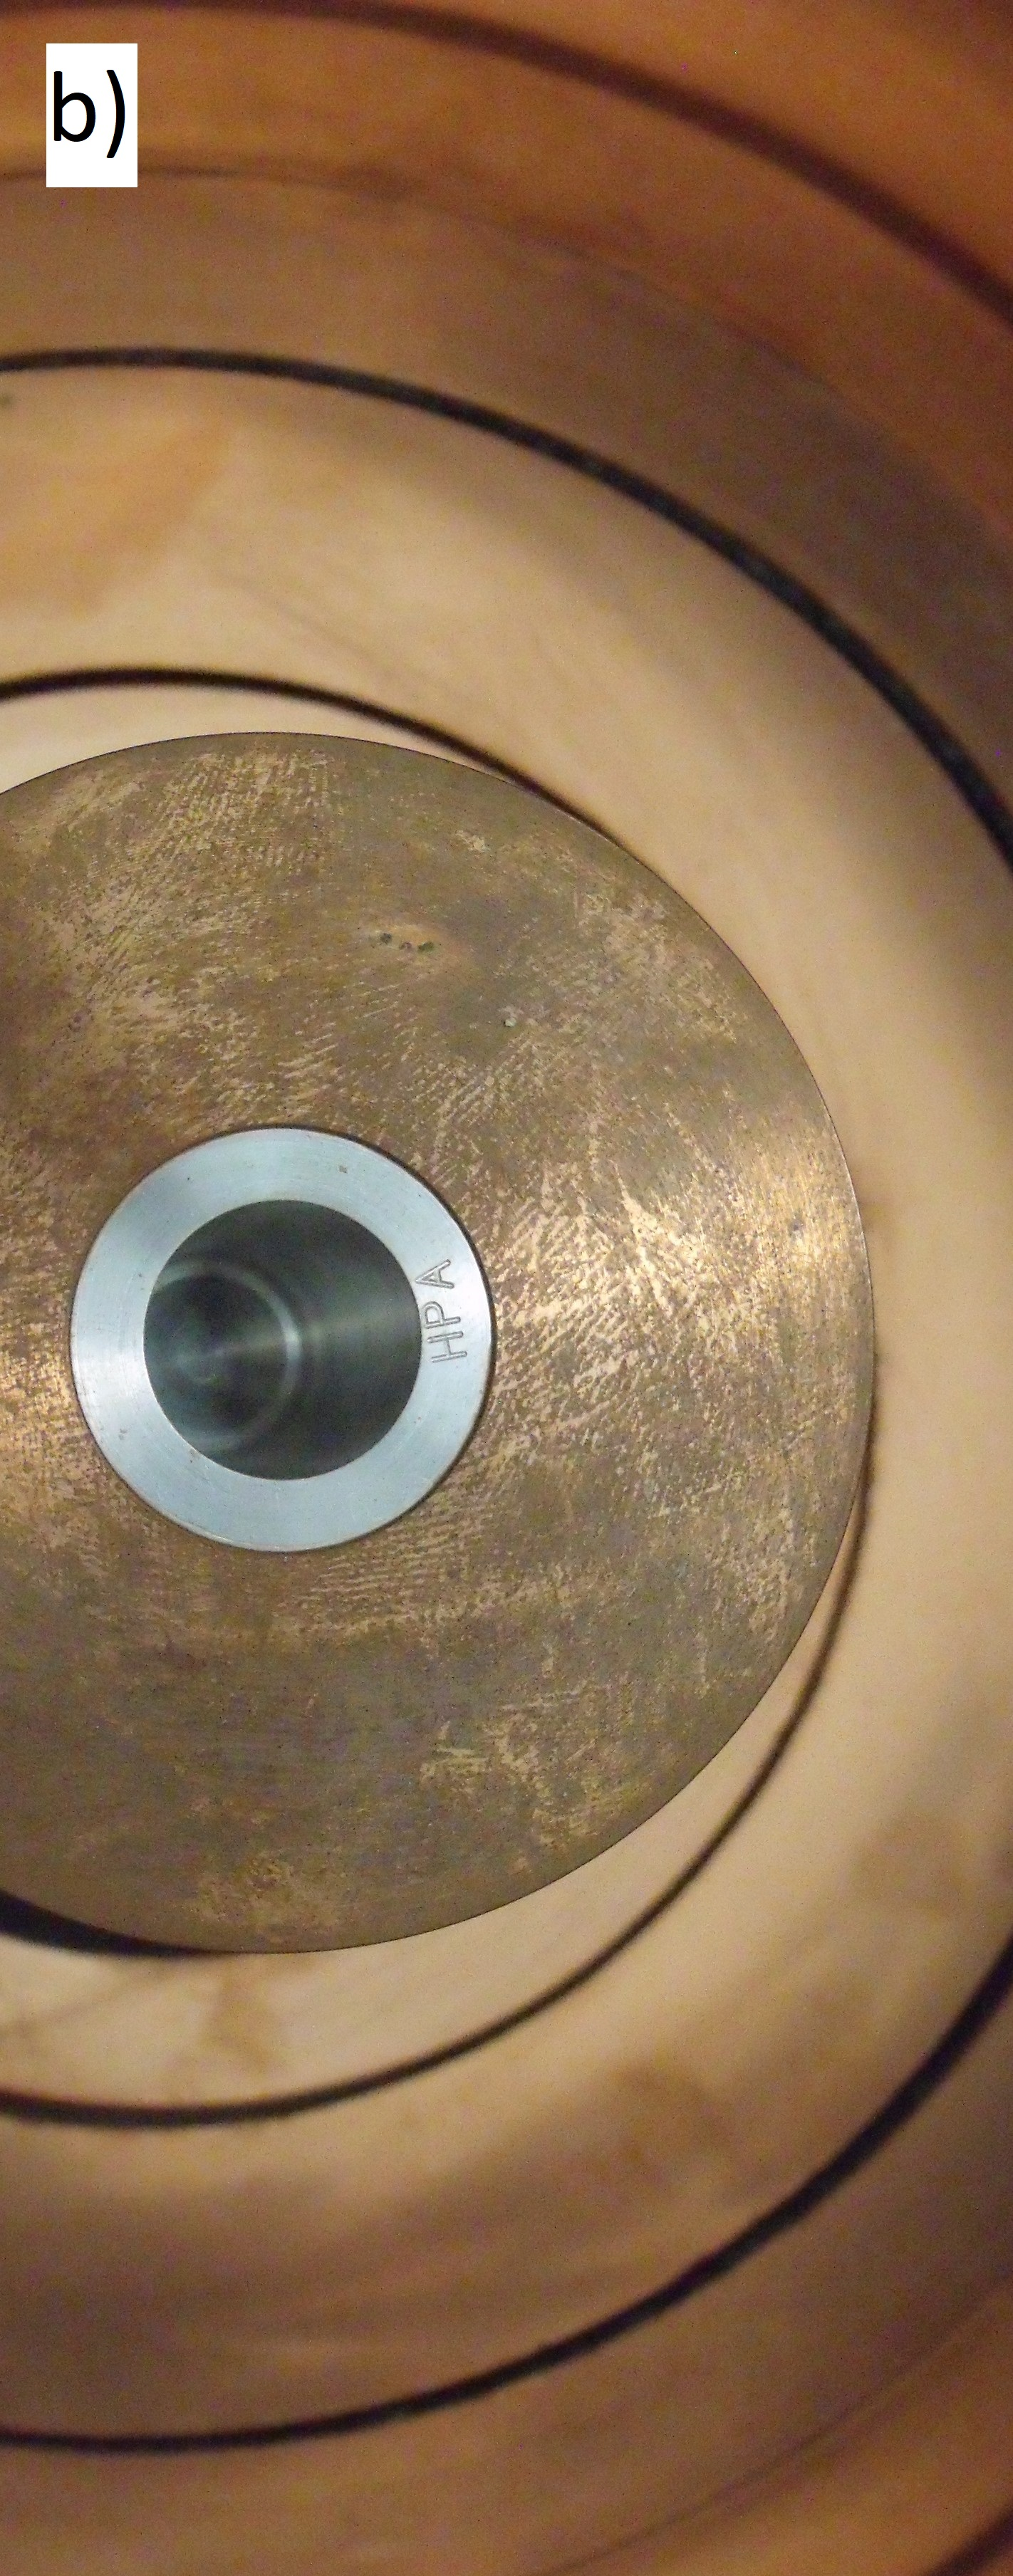
\includegraphics[height=0.45\textheight]{Imagenes/DSCF1886.jpg}
			\caption{\justifying Sistema de espectrometría de rayos gamma.}\label{Fig-G1System}
\end{figure}
		\end{column}
		\begin{column}{0.48\textwidth}  
			\begin{itemize}
			\justifying
			\item Detectores de germanio hiper-puro tipo pozo, marca ORTEC y modelos GWL-120-15-5, GWL-120-15-LB-AWT, GWL-150-15-LB-AWT. 
			\item Blindaje pasivo cilíndrico con $\sim$ 10 cm de plomo de bajo fondo y dos capas de Cu y Sn.
			\item Sistema de refrigeración equipo MÖBIUS Recycler, ORTEC.
			\item Electrónica asociada: DSPEC jr 2.0, ORTEC.
			\end{itemize}
		\end{column}
	\end{columns}
\end{frame}

\begin{frame}{Eficiencia}
	\begin{columns}
		\begin{column}{0.53\textwidth}
			\justifying
			\begin{equation}
				\epsilon = \dfrac{\text{Números de eventos registrados}}{\text{Número de eventos emitidos}},
			\end{equation}
			\begin{equation}
				\epsilon(E) = \epsilon_{\text{intríseca}}(E)\cdot \epsilon(\Omega)\cdot\text{\hyperlink{TCSC}{\beamerbutton{TCSC}}}\cdot \eta(E), 
			\end{equation}
			donde $\eta(E):$ factor de autoabsorción.
			\\ \vspace{0.5cm}
			La actividad $A$ de un radionúclido se determina mediante la ecuación\footnotemark[1]
			\begin{equation}
				A = \dfrac{N(E) - B(E)}{\epsilon(E)\,f_\gamma(E)\,t} \propto \dfrac{1}{\epsilon(E)}
			\end{equation}
		\end{column}
		\begin{column}{0.45\textwidth}  
			\justifying
			\begin{figure}
			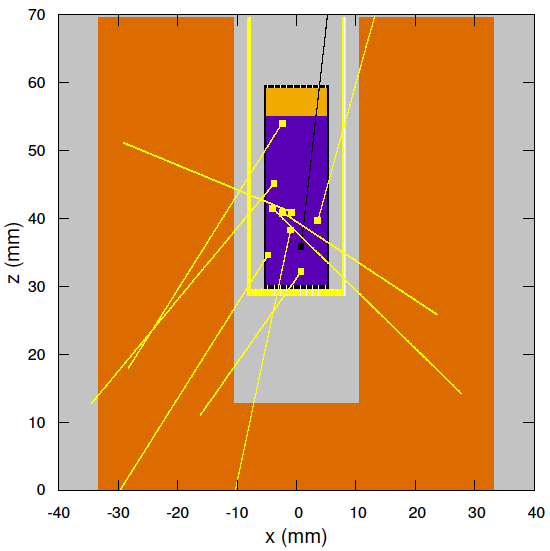
\includegraphics[width=1\textwidth]{Imagenes/ZY-2.png}
			\end{figure}
		\end{column}
	\end{columns}
\begin{center}
Las correcciones en la $\epsilon$ afecta directamente a $A$.	
\end{center}
\footnotetext[1]{Olivares et al., Applied Radiation and Isotopes, 130:34 – 42, 2017.}
\end{frame}

\begin{frame}{Calibraciones}
	\justifying Se utiliza una \textbf{solución acuosa patrón de emisores gamma} y un material de referencia \textbf{Uranio - Torio ORE DL1a} para realizar las calibraciones.
	\begin{columns}
		\begin{column}{0.48\textwidth}
			\begin{figure}
			\centering
			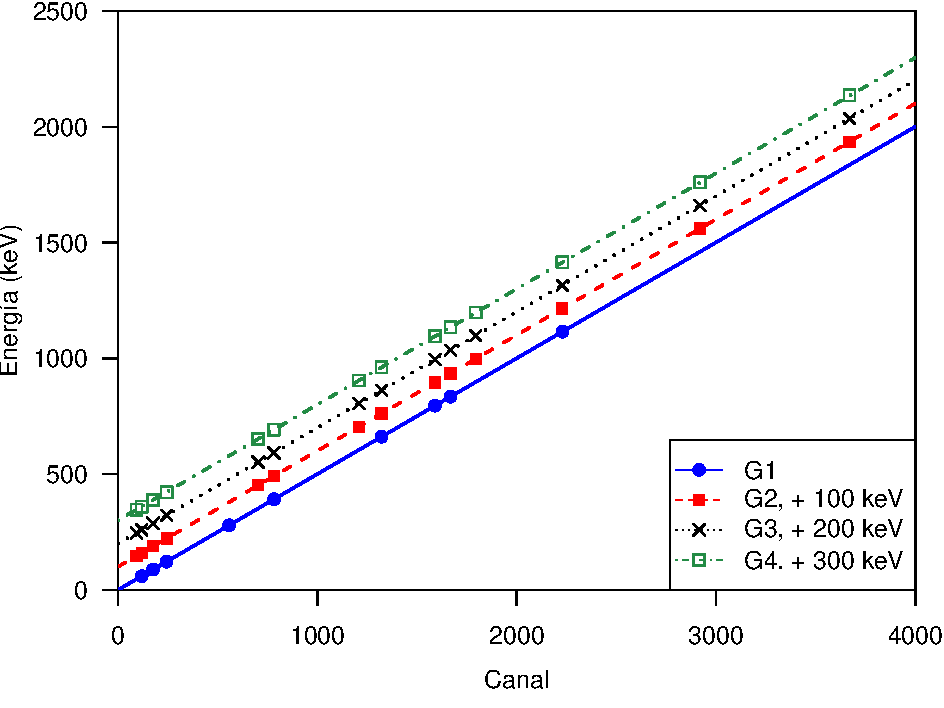
\includegraphics[width=1\textwidth]{Imagenes/Calibraciones_Canal_Energia.pdf}
			\caption{\justifying Calibración canal-energía para los sistemas de espectrometría de rayos gamma.}\label{Fig-Cal-Canal-Energia}
			\end{figure}
		\end{column}
		\begin{column}{0.48\textwidth}  
			\begin{figure}
			\centering
			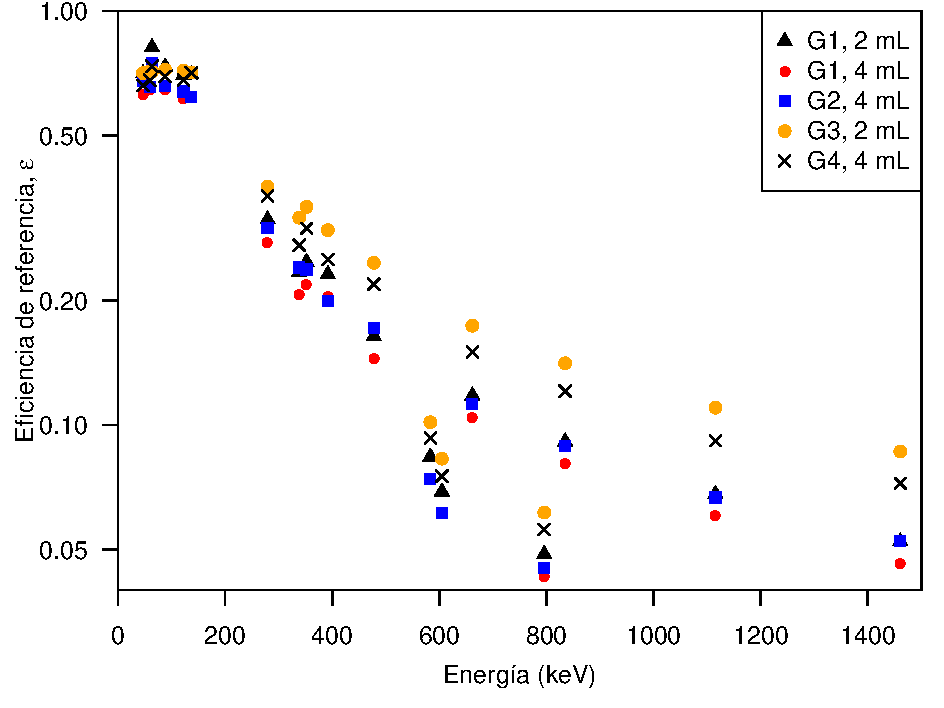
\includegraphics[width=1\textwidth]{Imagenes/Eficiencia_agua.pdf}
			\caption{\justifying Eficiencia de referencia para diferentes detectores y geometrías (2 mL y 4 mL) del LGIG.}\label{Fig-EficienciaAgua}
			\end{figure}
		\end{column}
	\end{columns}
\end{frame}

\begin{frame}{Función de transferencia}

\begin{figure}
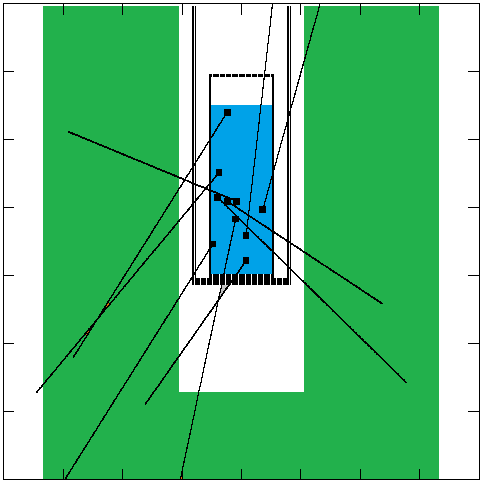
\includegraphics[width=0.33\textwidth]{Imagenes/ZY-Paint.png}

\includegraphics[width=0.05\textwidth]{Imagenes/Flecha.jpg}
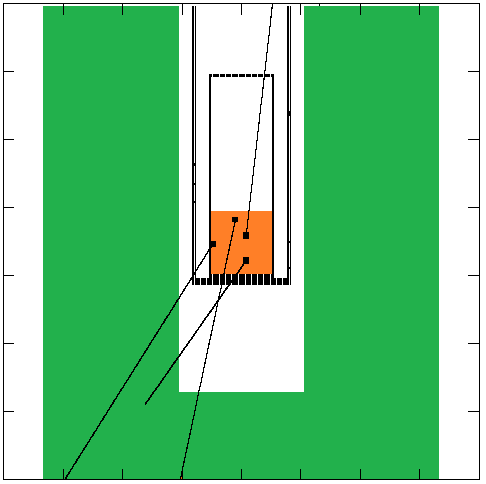
\includegraphics[width=0.33\textwidth]{Imagenes/ZY-Paint2.png}
\end{figure}
\begin{center}
\begin{tabular}{ccc}
Eficiencia y composición  & $\rightarrow$ & Eficiencia para una composición  \\
de referencia & & y geometría diferente 
\end{tabular}
\end{center}
			\begin{equation}
				\epsilon = \dfrac{\overline{\Omega}}{\overline{\Omega}_\text{referencia}}\,\epsilon_\text{referencia},
			\end{equation}
\end{frame}

\begin{frame}{Función de transferencia}
	\begin{columns}
		\begin{column}{0.58\textwidth}
			\justifying
			ANGLE permite el cálculo de la eficiencia $\epsilon$ mediante \textbf{funciones de transferencia}, 
			\begin{equation}
				\epsilon = \dfrac{\overline{\Omega}}{\overline{\Omega}_\text{referencia}}\,\epsilon_\text{referencia},
			\end{equation}
partiendo de una eficiencia de referencia $\epsilon_\text{referencia}$, donde 
			\begin{equation}
				\overline{\Omega} = \int_{V_S, S_D}\,\displaystyle F_{\text{atenuación}}\,F_{\text{efectivo}} \dfrac{\overrightarrow{TP}\cdot\hat{n}}{|\overrightarrow{TP}|^3}\,d\sigma.
			\end{equation}
			\begin{center}
			$F_{\text{atenuación}}$ se relaciona con $\dfrac{\mu}{\rho}$.
			\end{center}
								\begin{columns}
			\begin{column}{0.2\textwidth}
			
\includegraphics[width=1\textwidth]{Imagenes/Atencion.png}
			\end{column}
			\begin{column}{0.8\textwidth} 
			 ¡Es necesario definir el \\ \textbf{100 \%} de las composiciones!
			\end{column}
			\end{columns}
		\end{column}
		\begin{column}{0.38\textwidth}  
			\begin{figure}
			\centering
			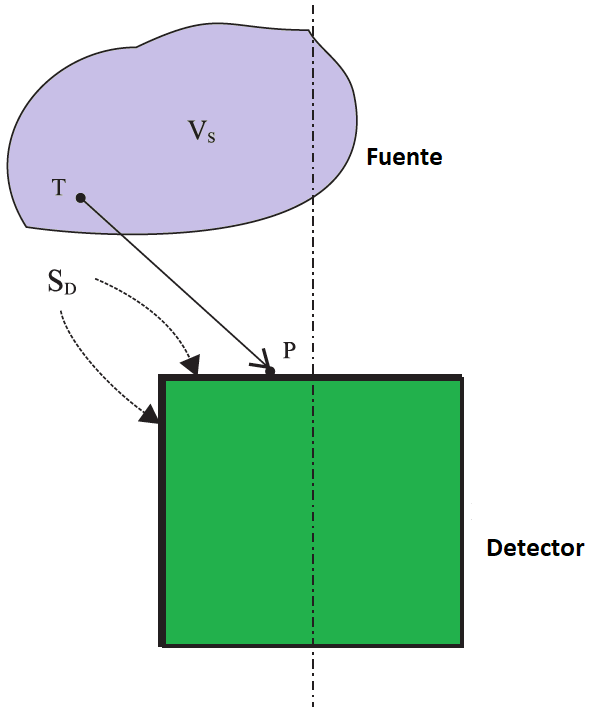
\includegraphics[width=1\textwidth]{Imagenes/EffectiveSolidAngle-3.png}
			\caption{\justifying Variables involucradas en el cálculo de $\overline{\Omega}$.}
			\end{figure}
		\end{column}
	\end{columns}
\end{frame}

\begin{frame}{Análisis elemental: espectrometría de fluorescencia de rayos X, XRF}
	\begin{columns}
		\begin{column}{0.58\textwidth}
			\begin{figure}
			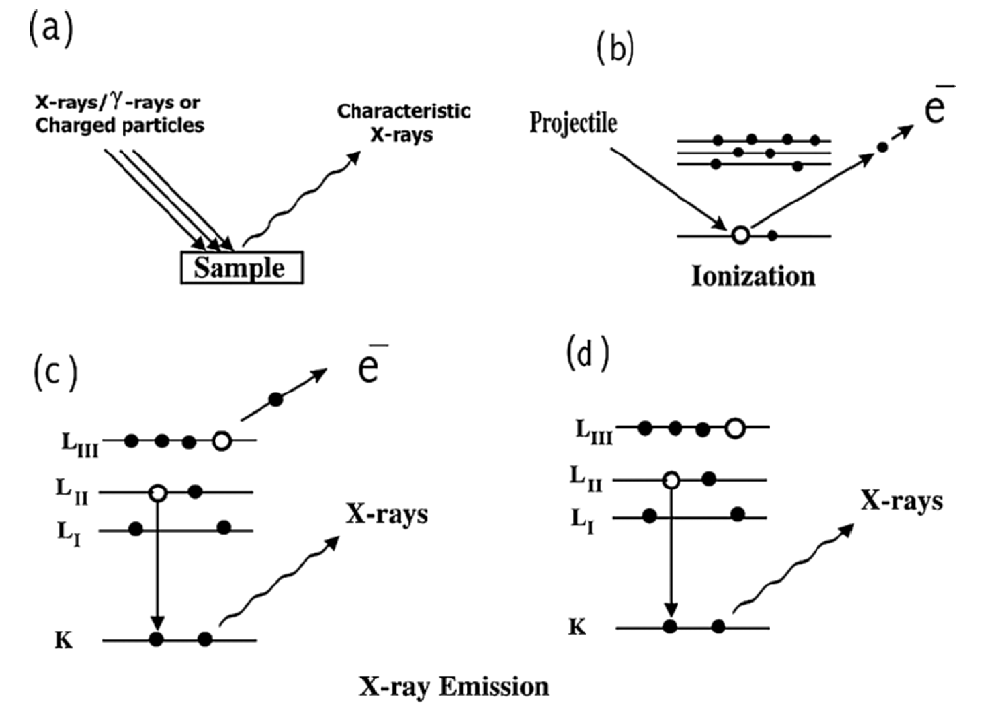
\includegraphics[width=0.8\textwidth]{Imagenes/XRF-Book.png}
			\caption{Representación esquemática de la emisión de rayos X\footnotemark[1].}
			\end{figure}
			\justifying En el LGIG se mide la concentración elemental para $Z>10$. 
			\\
			\vspace{0.5cm}
			La cantidad de masa requerida es de \textbf{2 a 4 g}.
		\end{column}
		\begin{column}{0.38\textwidth}  
			\begin{figure}
			\centering
			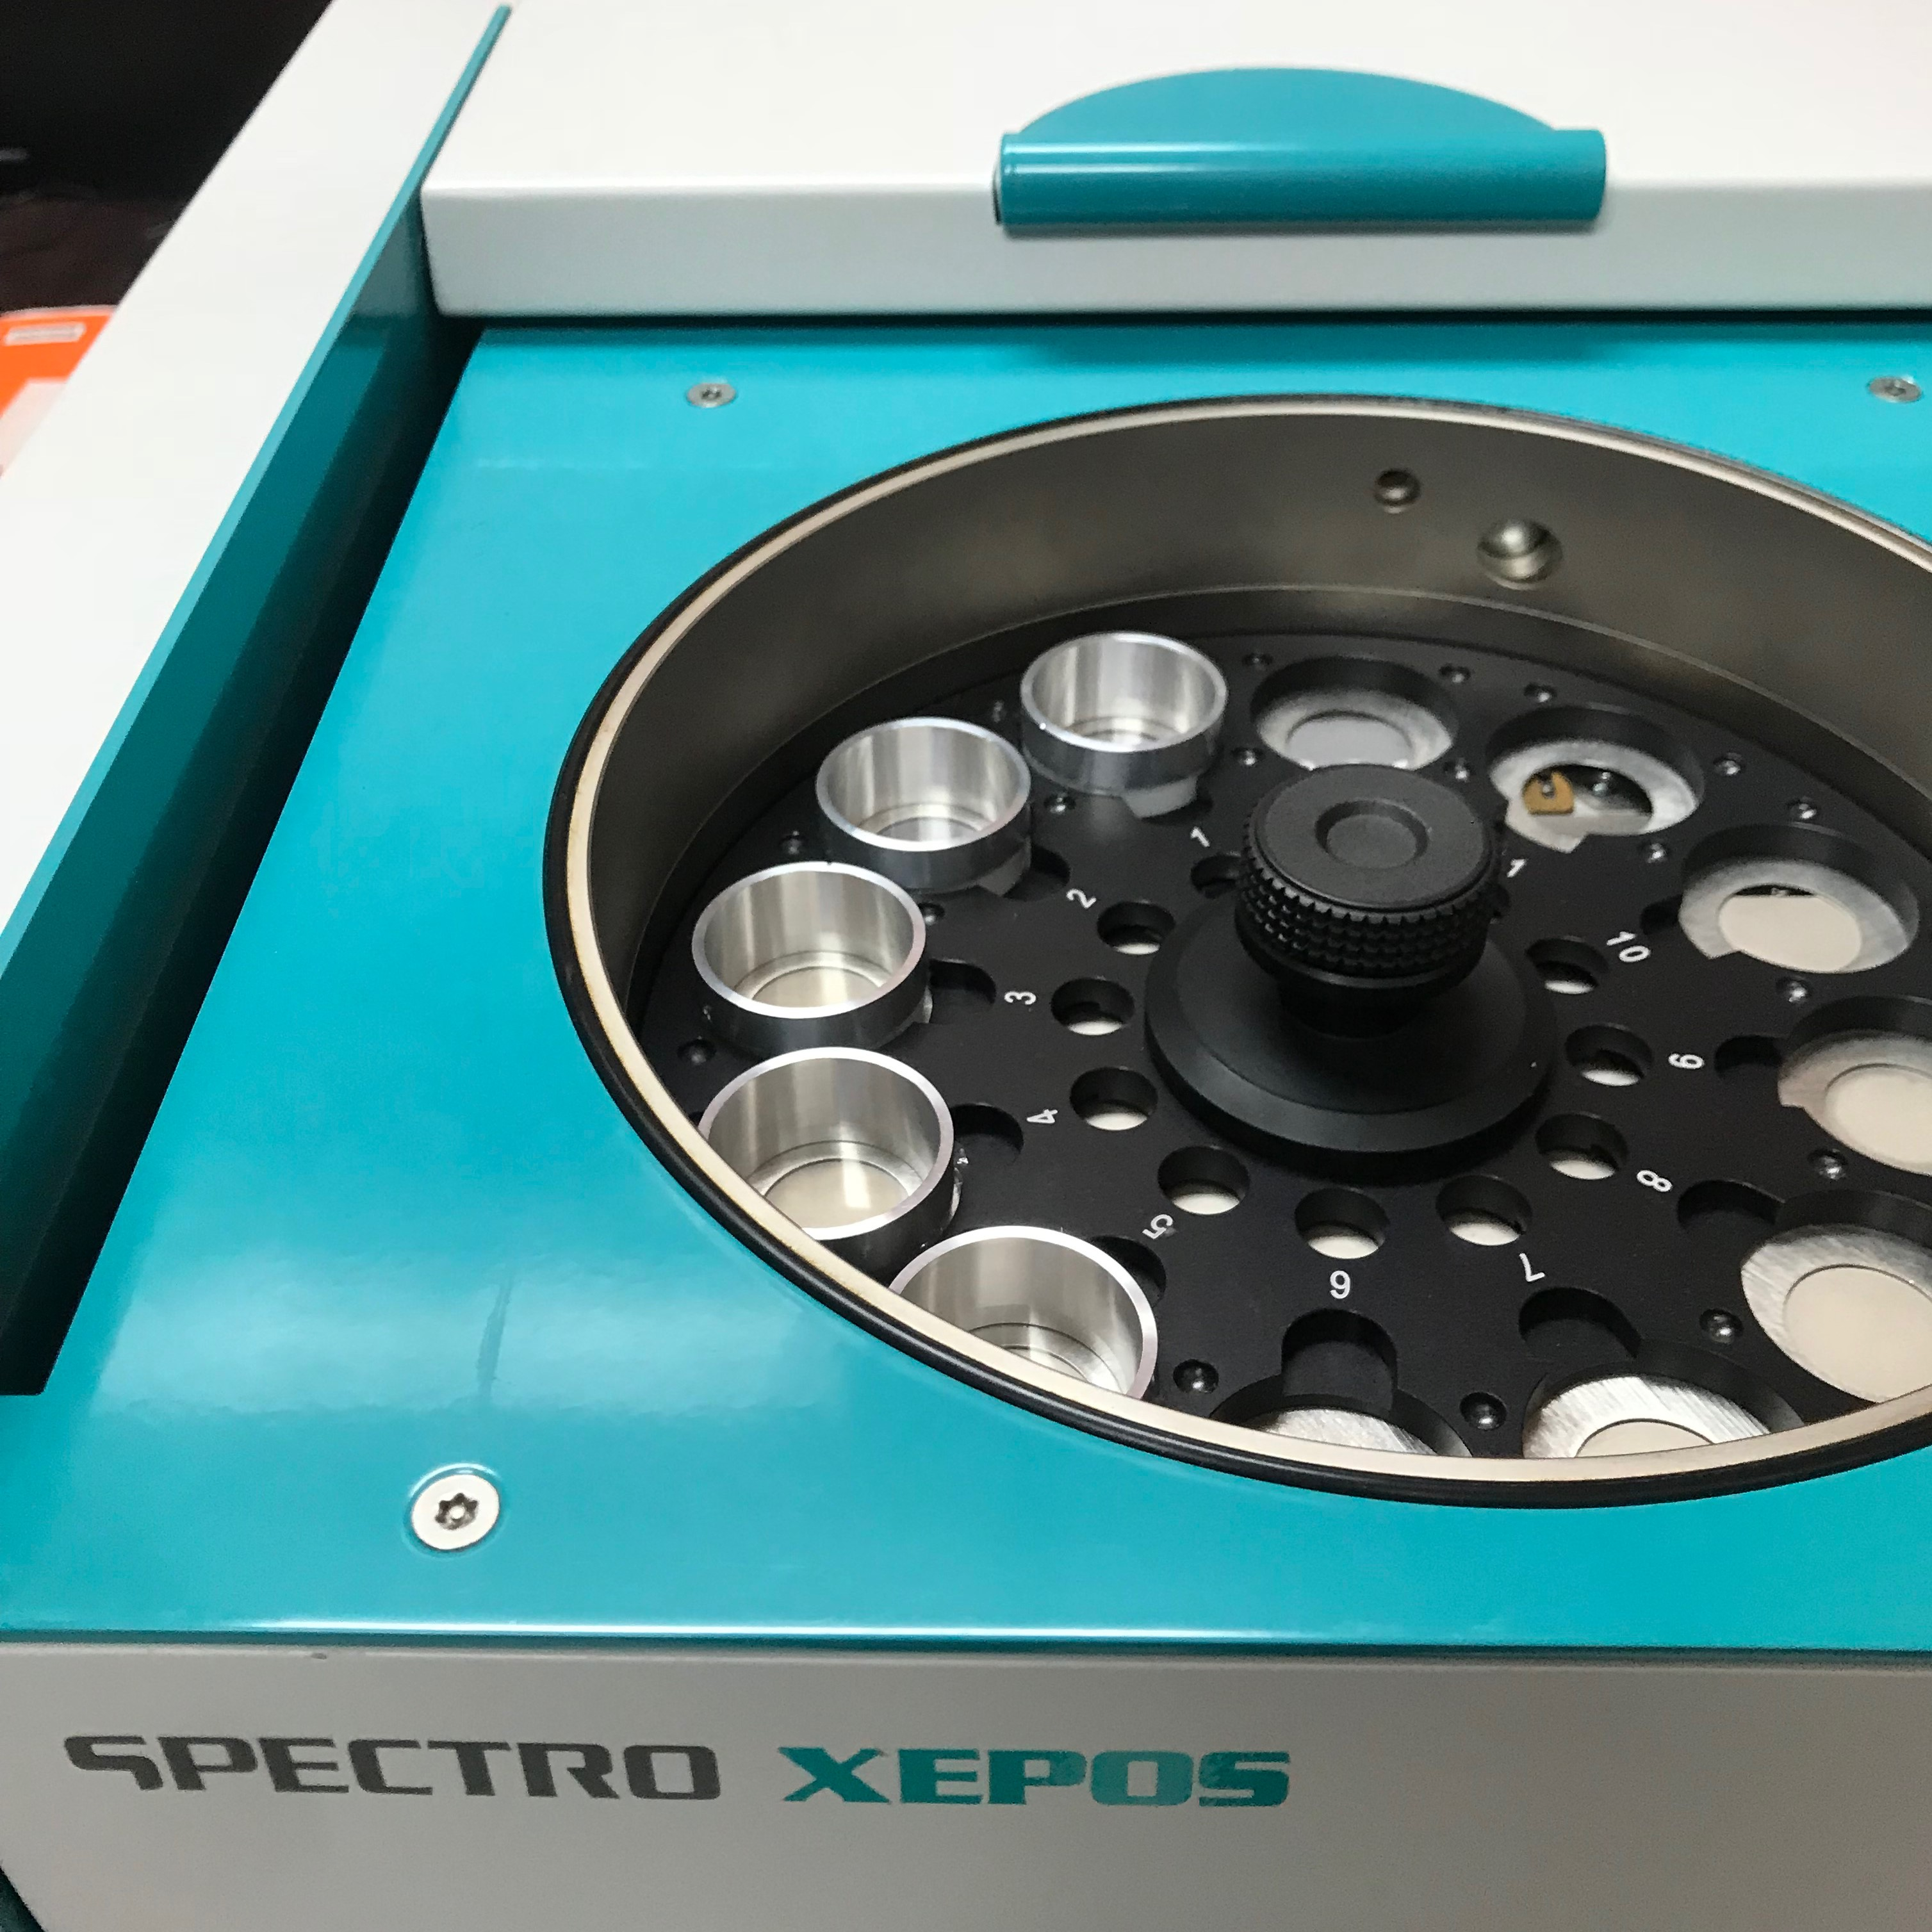
\includegraphics[width=1\textwidth]{Imagenes/XEPOS.jpg}
			\caption{\justifying Vista superior equipo de fluorescencia de rayos X, \textit{SPECTRO XEPOS III}, del LGIG.}
			\end{figure}
		\end{column}
	\end{columns}
	\footnotetext[1]{\textit{Atomic and Nuclear Analytical Methods}, H.R. Verma, Springer, 2007.}
\end{frame}

\begin{frame}{Análisis elemental: carbono y nitrógeno, C-N}
	\begin{figure}
		\centering
		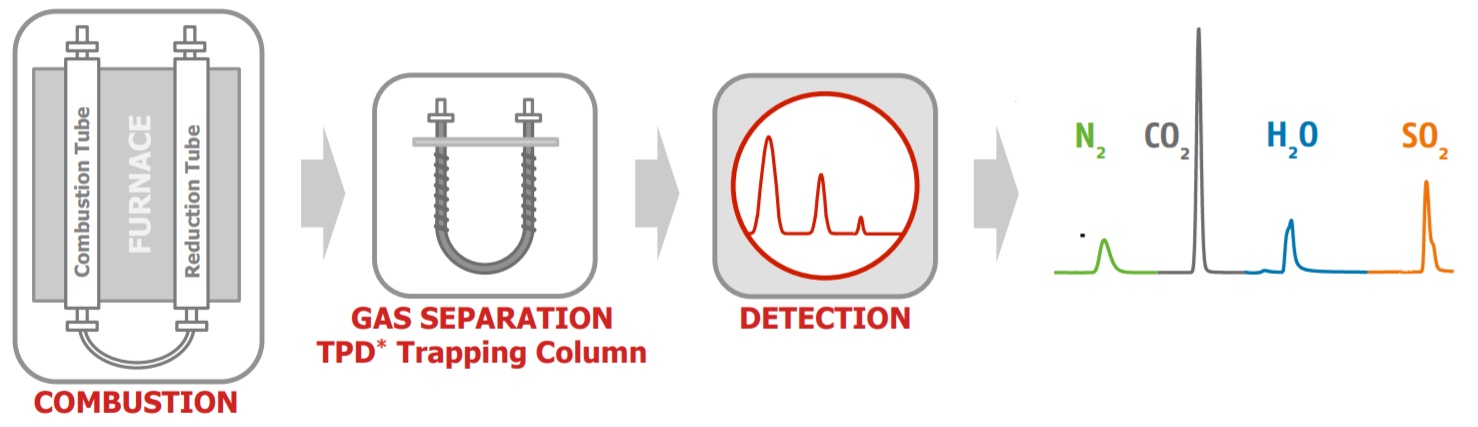
\includegraphics[width=0.5\textwidth]{Imagenes/C-N-Detection.png}
		\caption{\justifying Procedimientos para el análisis C-N: combustión, separación de gases y detección\footnotemark[1].}
	\end{figure}
	\begin{columns}
		\begin{column}{0.68\textwidth}
			\justifying
La medición se realiza mediante cromatografía de gases y un detector de termoconductividad.
\\ \vspace{0.5cm}
			La cantidad de masa necesaria es $\sim$ 20 mg. 
			\\\vspace{0.5cm}
			La incertidumbre en la medición se calcula a través de triplicados.
		\end{column}
		\begin{column}{0.3\textwidth}  
		\begin{figure}
			\centering
			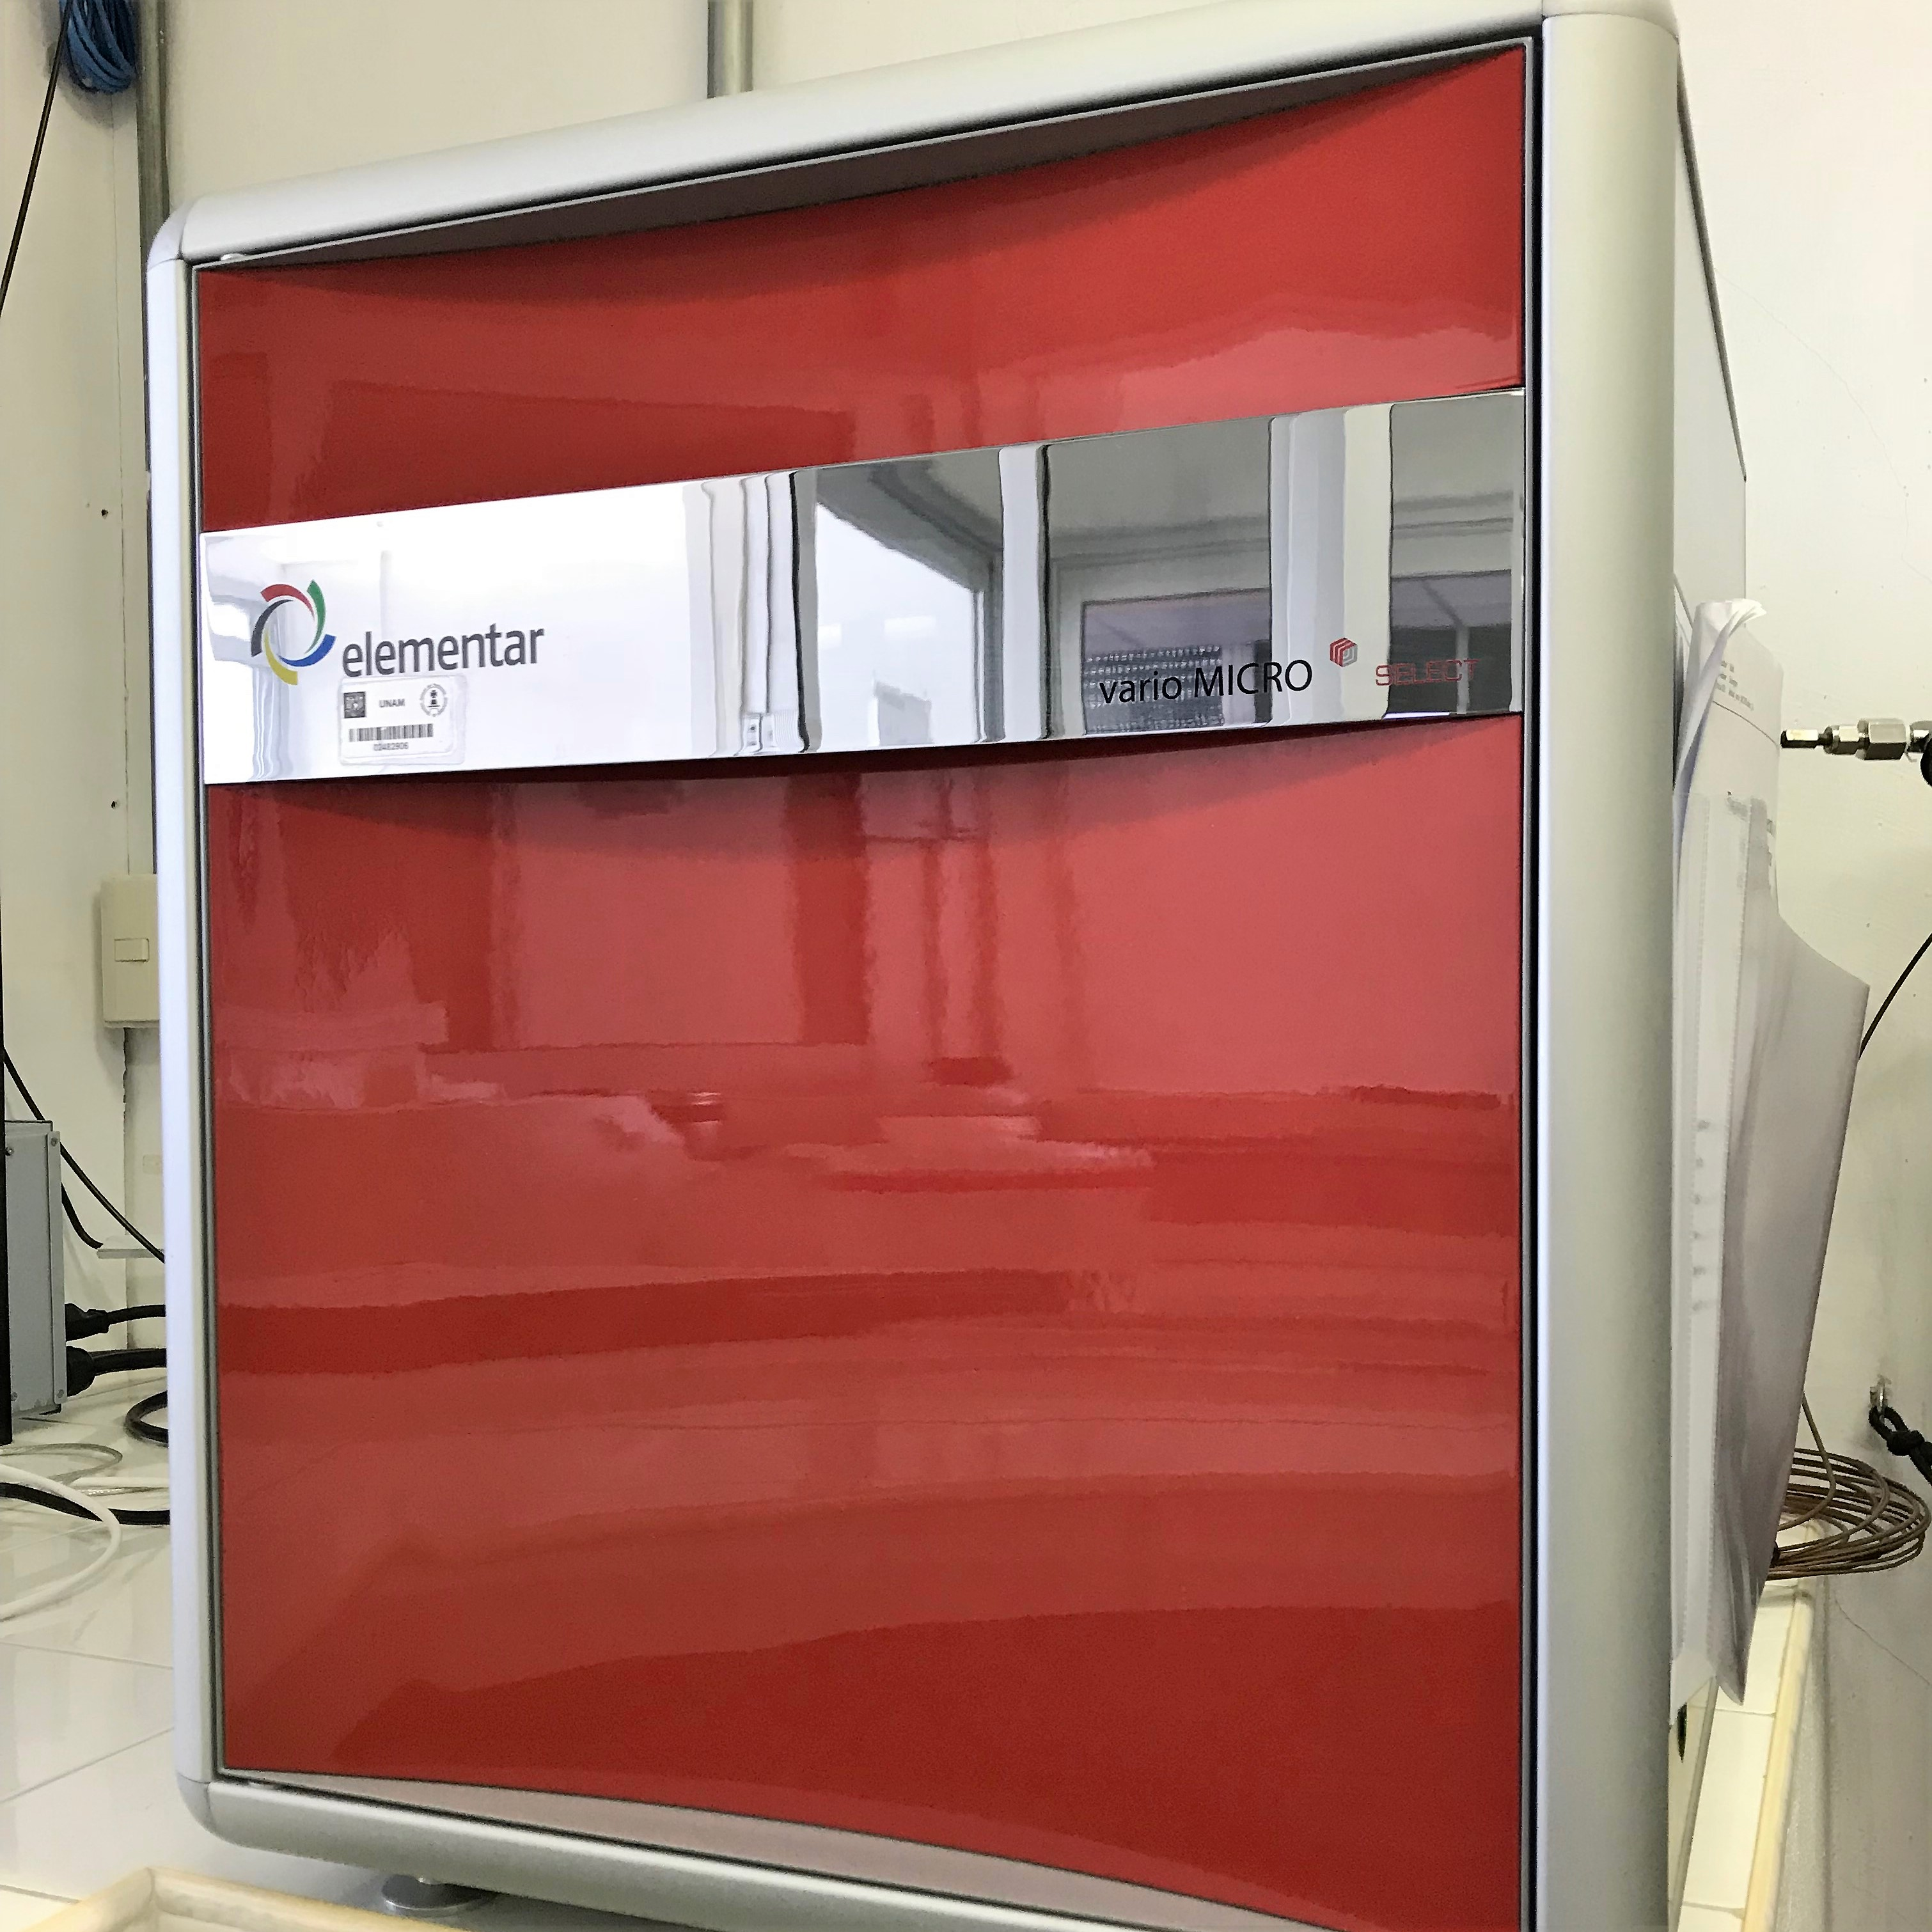
\includegraphics[width=0.8\textwidth]{Imagenes/Elementar.jpg}
			\caption{\justifying Analizador elemental de C-N \textit{Vario Micro Cube, Elementar}.}
		\end{figure}
		\end{column}
	\end{columns}
\footnotetext[1]{\textit{Flyer vario MICRO cube}, marca Elementar.}
\end{frame}

\begin{frame}{100 \% de la composición elemental}
	\justifying
	\begin{eqnarray}
		100 \% \text{ de la composición}	&=& X_\text{medido} + X_\text{desconocido}, \\
		X_\text{medido} 			&=& \text{XRF(Na, Mg, ..., U) + C-N.} 
	\end{eqnarray}
	Se desconoce elementos ligeros, entre los que se destacan H y O porque 	
	son constituyentes relevantes de
\begin{itemize}
\item la materia orgánica (fundamentalmente C, H y O), y
\item de los carbonatos (Ca, C y O). 
\end{itemize}	
	\begin{equation}
		 X_\text{desconocido} = \text{hidrógeno + oxígeno},
	\end{equation}
	\begin{figure}
		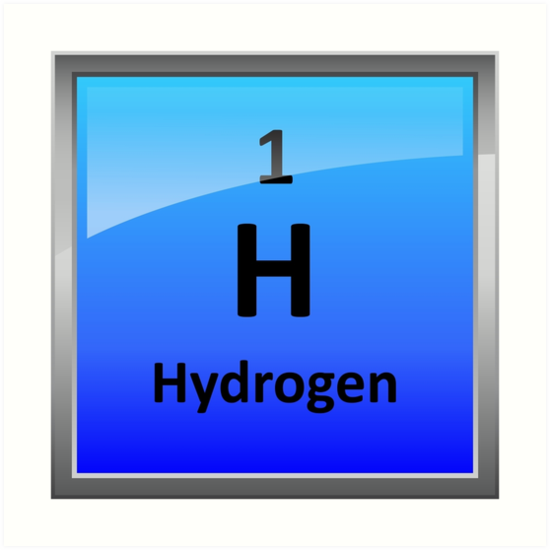
\includegraphics[height=0.15\textheight]{Imagenes/Hidrogeno.png}
		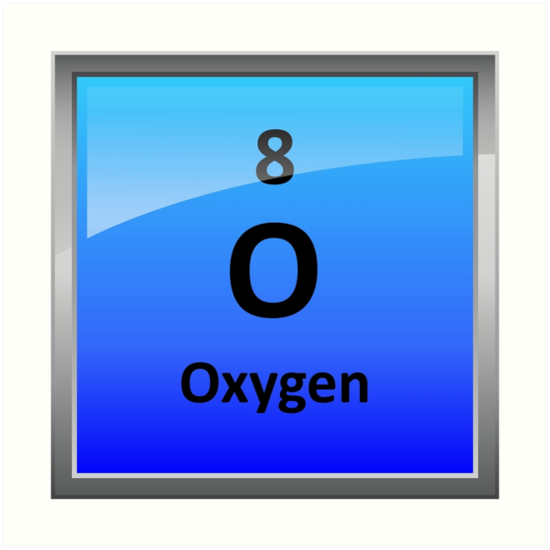
\includegraphics[height=0.15\textheight]{Imagenes/Oxigeno.png}
	\end{figure}
\end{frame}

\begin{frame}{Composición de referencia y corregida}

	\begin{tabular}{rcl}
	\textbf{Composición de referencia} & : & agua, \\
	\textbf{Composición corregida} & : & XRF + C-N + Oxígeno + Hidrógeno. 
\includegraphics[scale=0.1]{Imagenes/CaritaFeliz2.jpg}
	\end{tabular}
	\\
	\vspace{0.5cm}
		\justifying   Las cantidades que se relacionan con las composiciones son
	\begin{itemize}
	\item la eficiencia $\epsilon$, 
	\item la actividad específica $A$ de un radionúclido, y
	\item los resultados del fechado
	\end{itemize}

	\begin{equation}\label{Eq-ActividadCorregida}
		A_\text{corr} = \dfrac{\epsilon_\text{ref}}{\epsilon_{\text{corr}}}\,A_\text{ref}.
	\end{equation}
\end{frame}

\begin{frame}{Objetivos}
\justifying \textbf{Objetivo general}: mejorar la cuantificación de los radionúclidos utilizados en el fechado de sedimentos recientes (\PbCero\, y \PbCuatro) a través de correcciones de densidad y composición para cada muestra analizada. \pause 
\\ 
\vspace{0.5cm}
\textbf{Objetivos específicos} 
\begin{itemize}
\justifying
\item Caracterizar los detectores de Ge: \hyperlink{Espectros}{\beamerbutton{fondos}}, calibración de canal-energía y eficiencia-energía.
\item Seleccionar núcleos sedimentarios representativos de diversos sistemas acuáticos mexicanos.
\item Determinar la composición elemental de algunas secciones y proponer su composición completa.
\item Desarrollar códigos de programación para la lectura e integración de los datos, así como para ejecutar de manera sistemática ANGLE.
\item Estudiar los efectos de la densidad y composición elemental sobre la eficiencia para energías de 46.54 keV y 351.93 keV.
\item Estudiar el efecto de las correcciones realizadas en las actividades y el fechado de los núcleos seleccionados en relación a los resultados con una composición de referencia. 
\end{itemize}
\end{frame}

\section{Resultados y discusión}

\begin{frame}{Zonas de Estudio}
	\begin{figure}
	\centering
	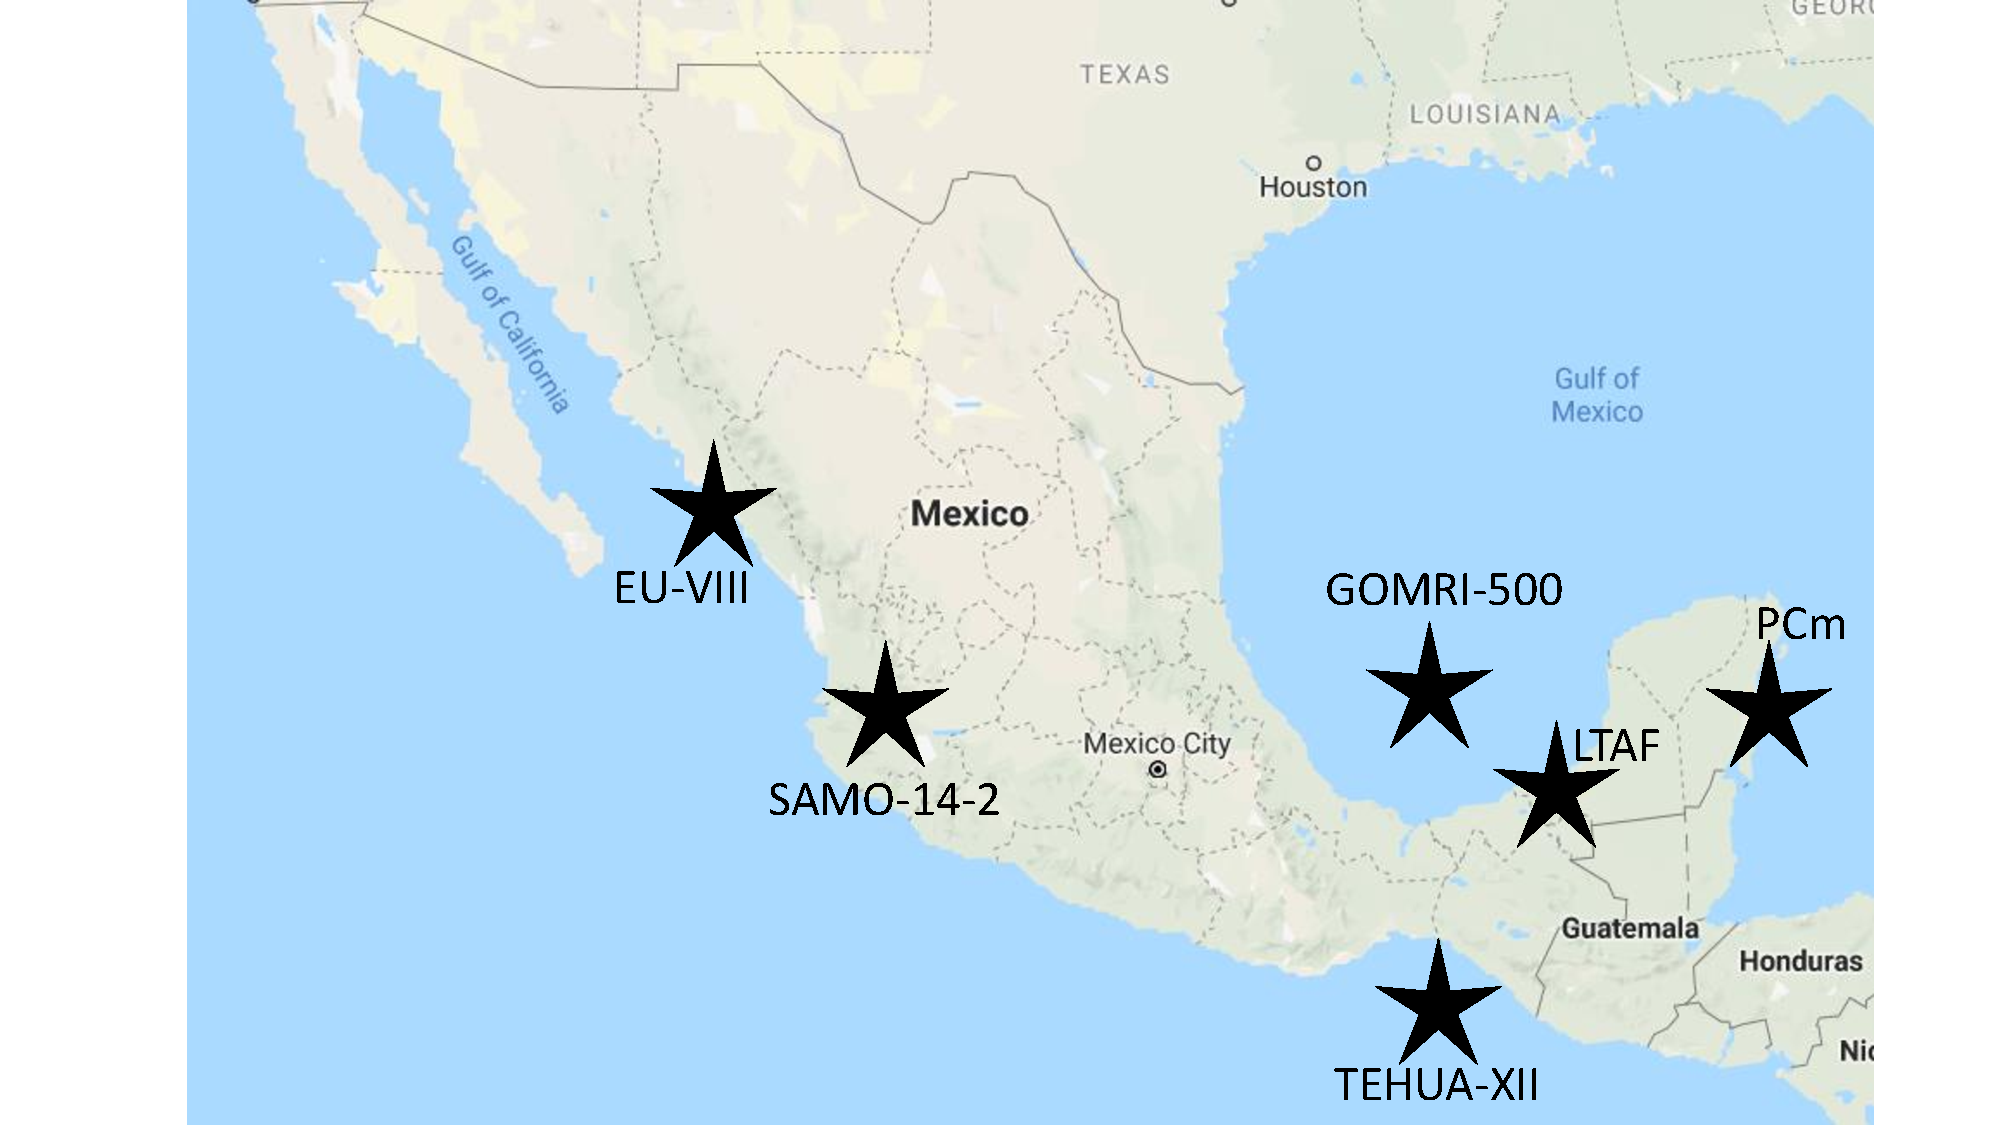
\includegraphics[width=0.9\textwidth]{Imagenes/Mapa_Nucleos_Seleccionados.pdf}
	\caption{Ubicación geográfica de los núcleos sedimentarios seleccionados para el presente trabajo.}
	\end{figure}
\end{frame}

\begin{frame}{Composición elemental medida de los núcleos sedimentarios}
	\begin{figure}
		\centering
		\includegraphics[width=0.48\textwidth]{Imagenes/XRF_Todos_Los_Nucleos_1-1.png}
		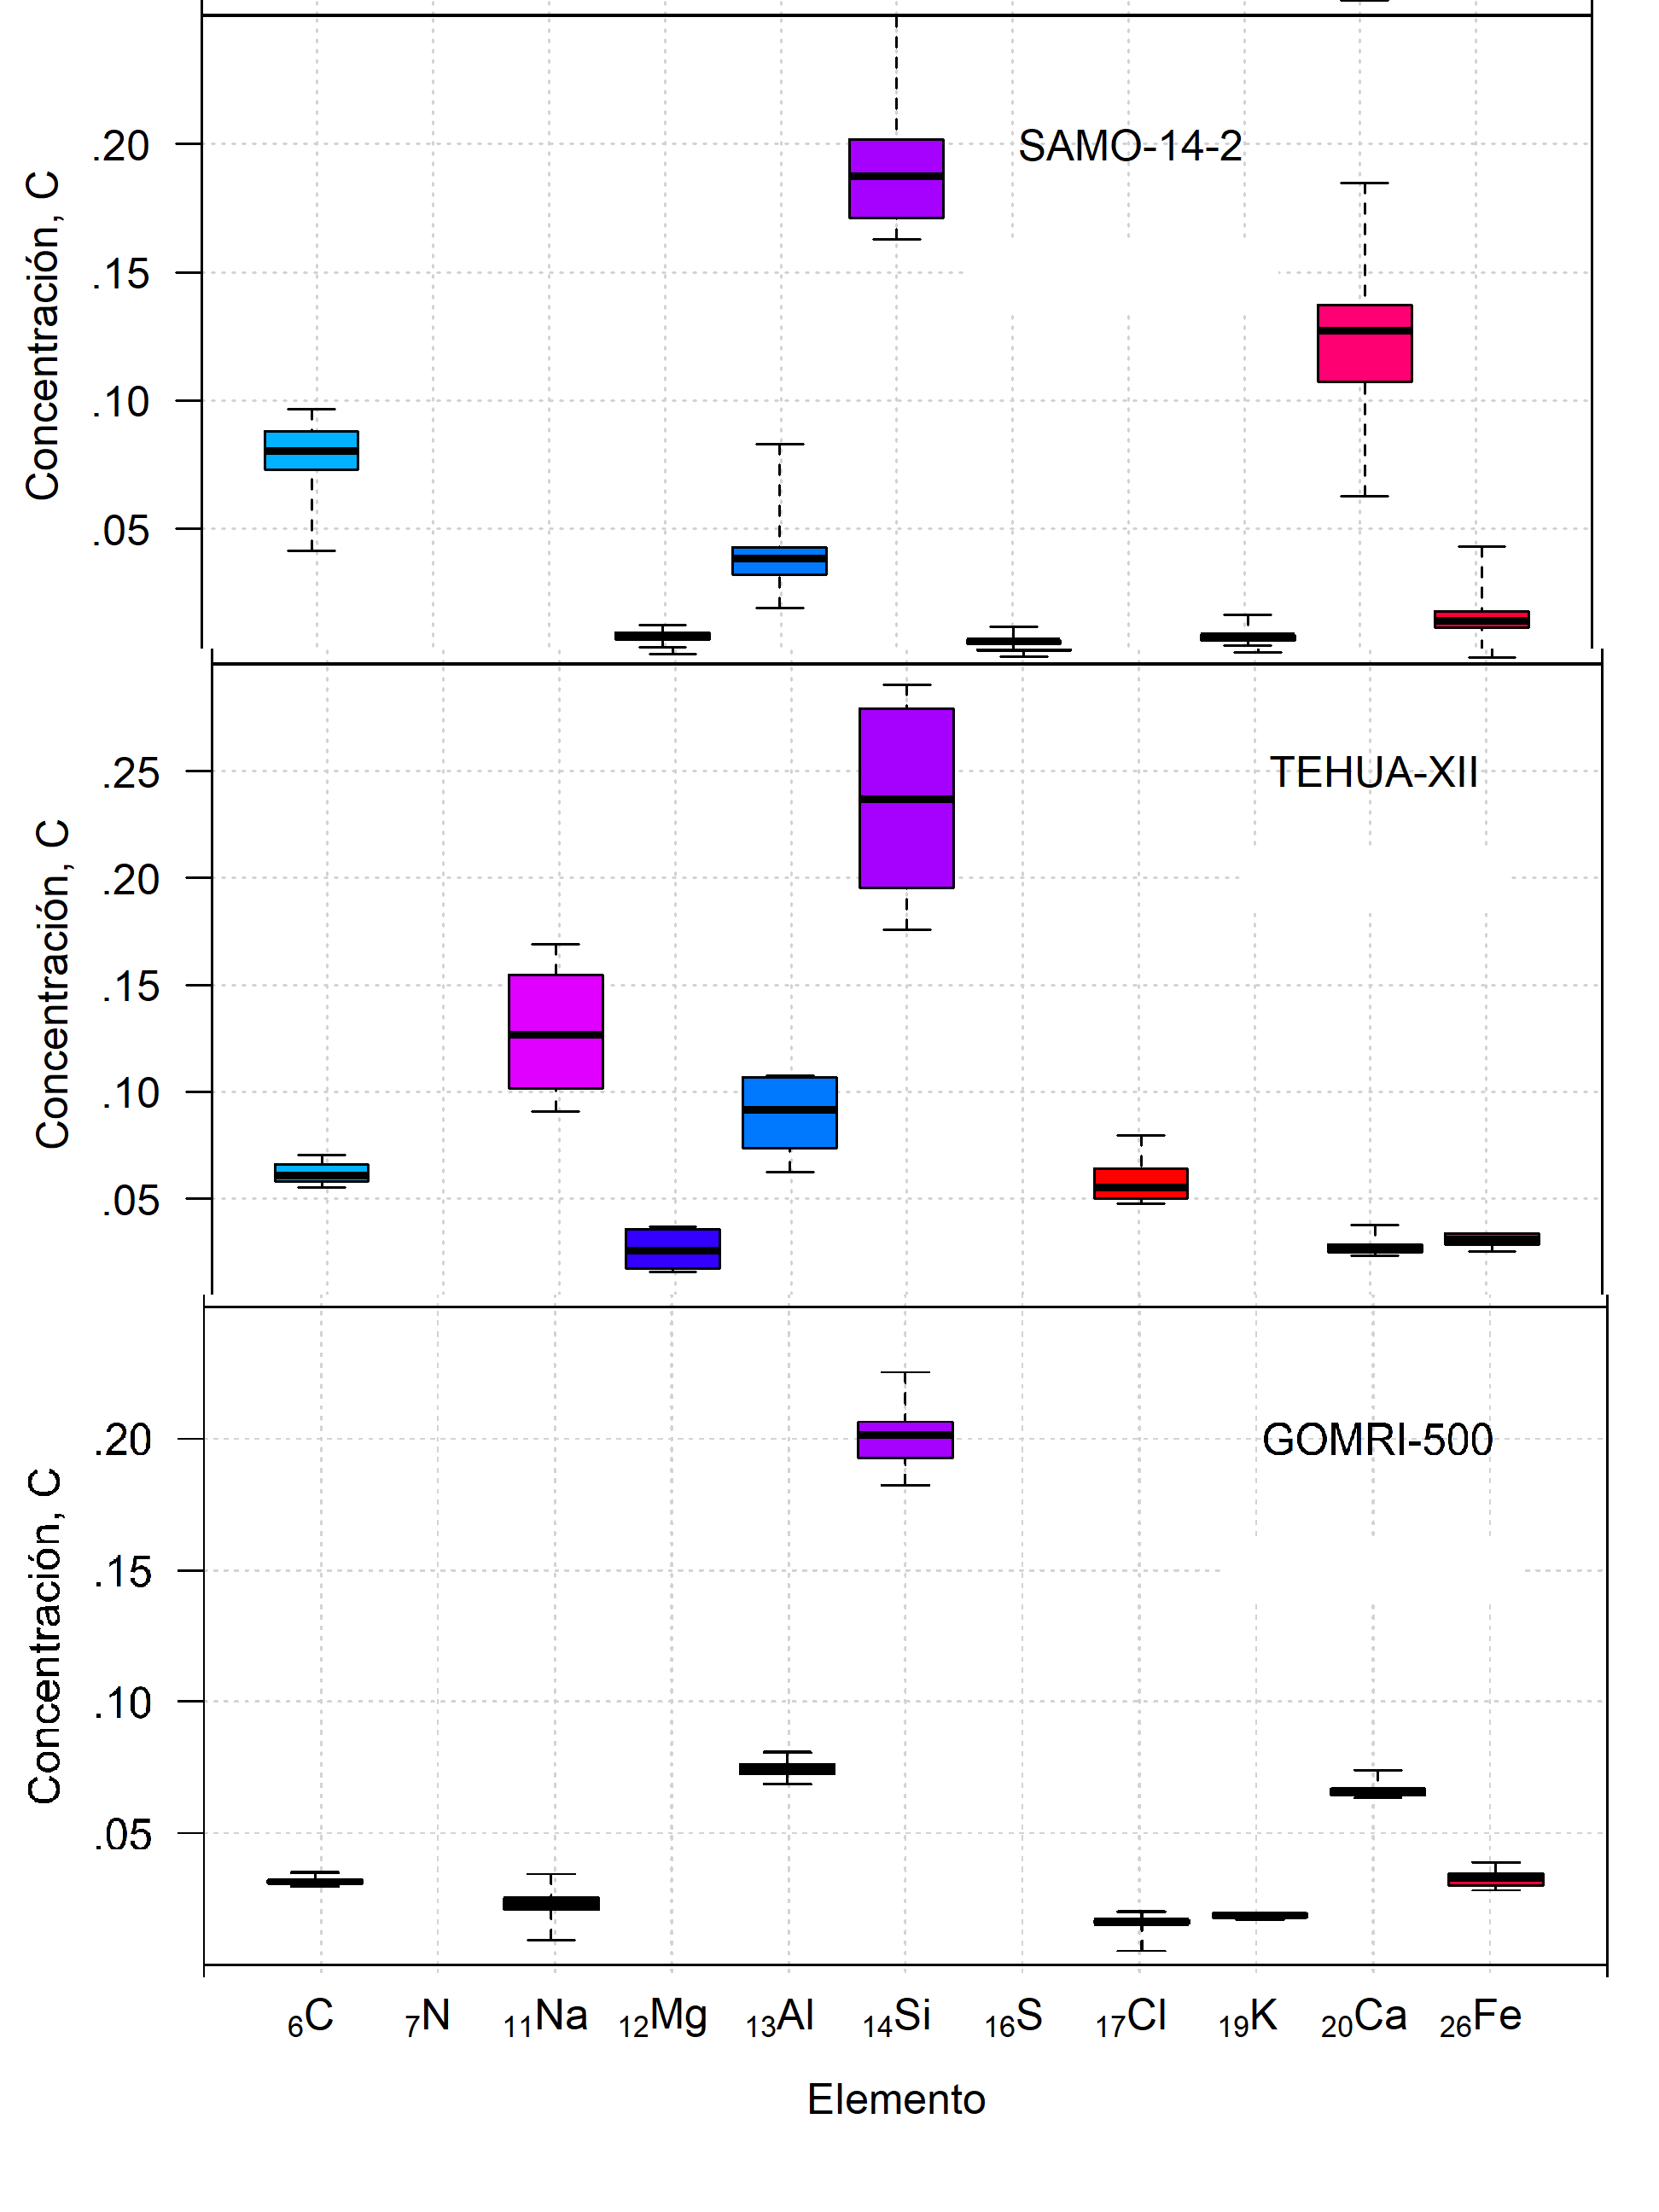
\includegraphics[width=0.48\textwidth]{Imagenes/XRF_Todos_Los_Nucleos_2-1.png}
	\end{figure}
\end{frame}

\begin{frame}{Composición elemental medida de los núcleos sedimentarios}
	\begin{figure}
		\centering
		\includegraphics[width=0.48\textwidth]{Imagenes/XRF_Todos_Los_Nucleos_1-2.png}
		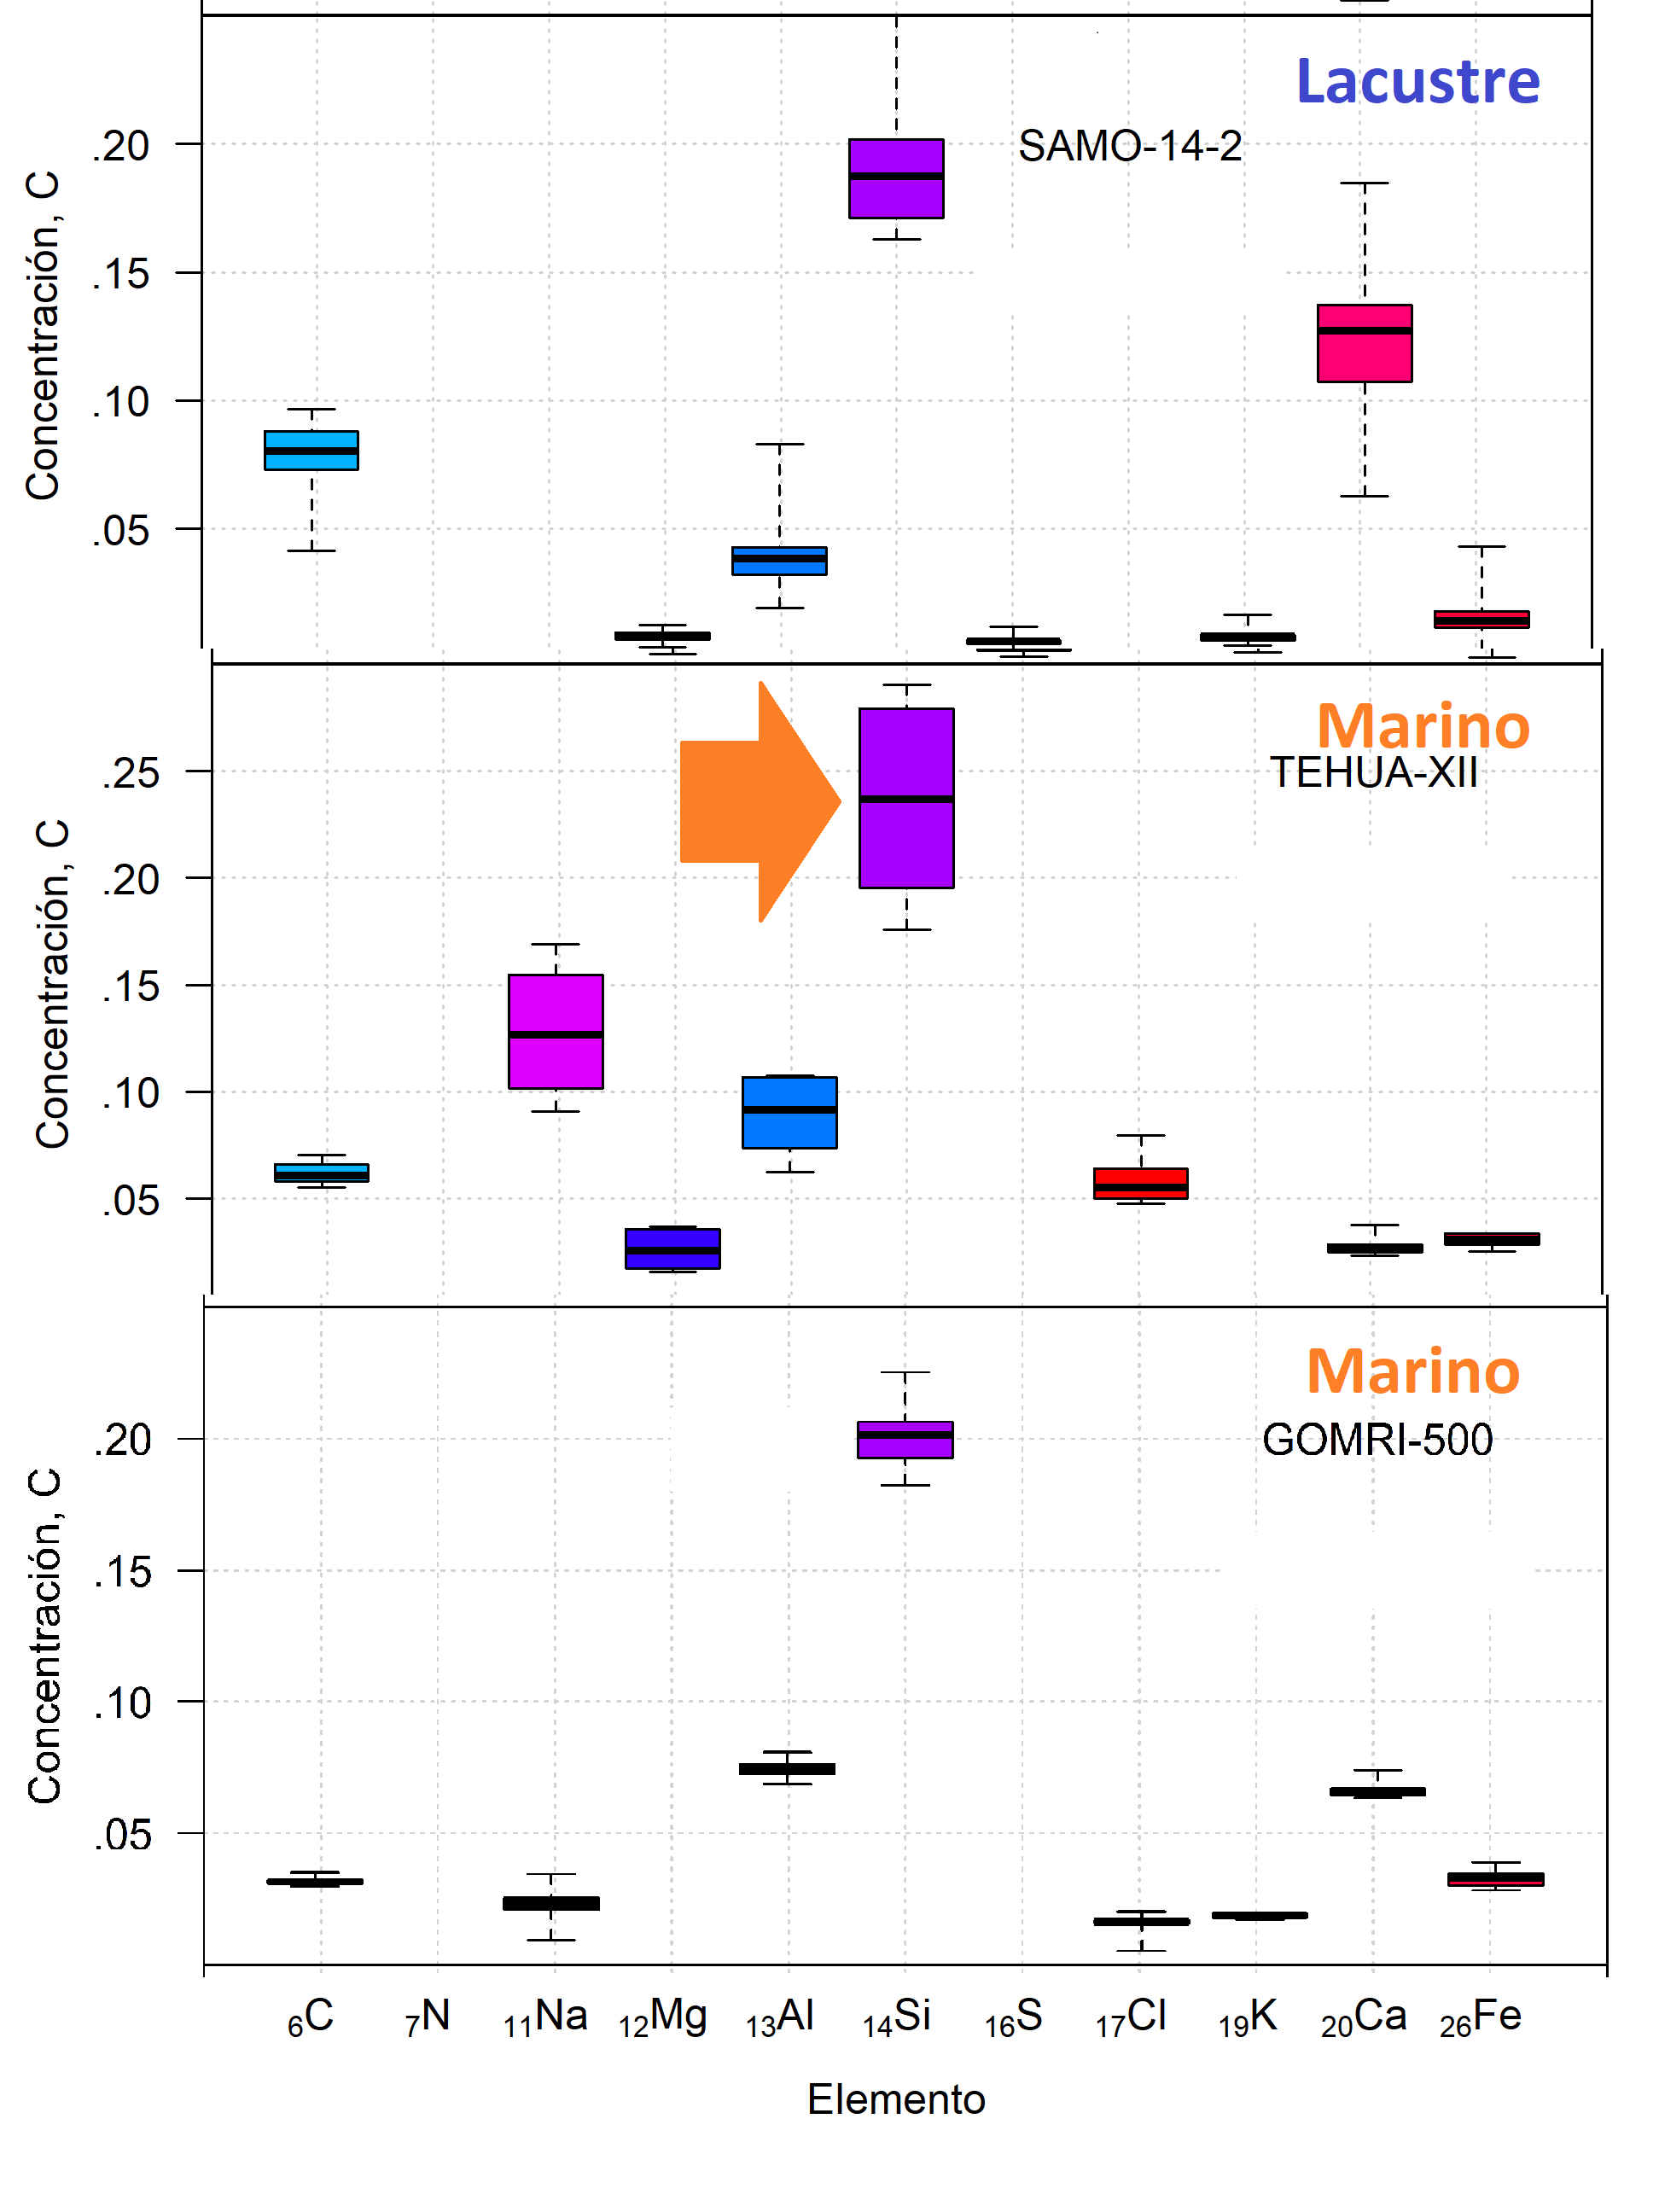
\includegraphics[width=0.48\textwidth]{Imagenes/XRF_Todos_Los_Nucleos_2-2.png}
	\end{figure}
\end{frame}

\begin{frame}{Composición elemental medida de los núcleos sedimentarios}
	\begin{figure}
		\centering
		\includegraphics[width=0.48\textwidth]{Imagenes/XRF_Todos_Los_Nucleos_1-3.png}
		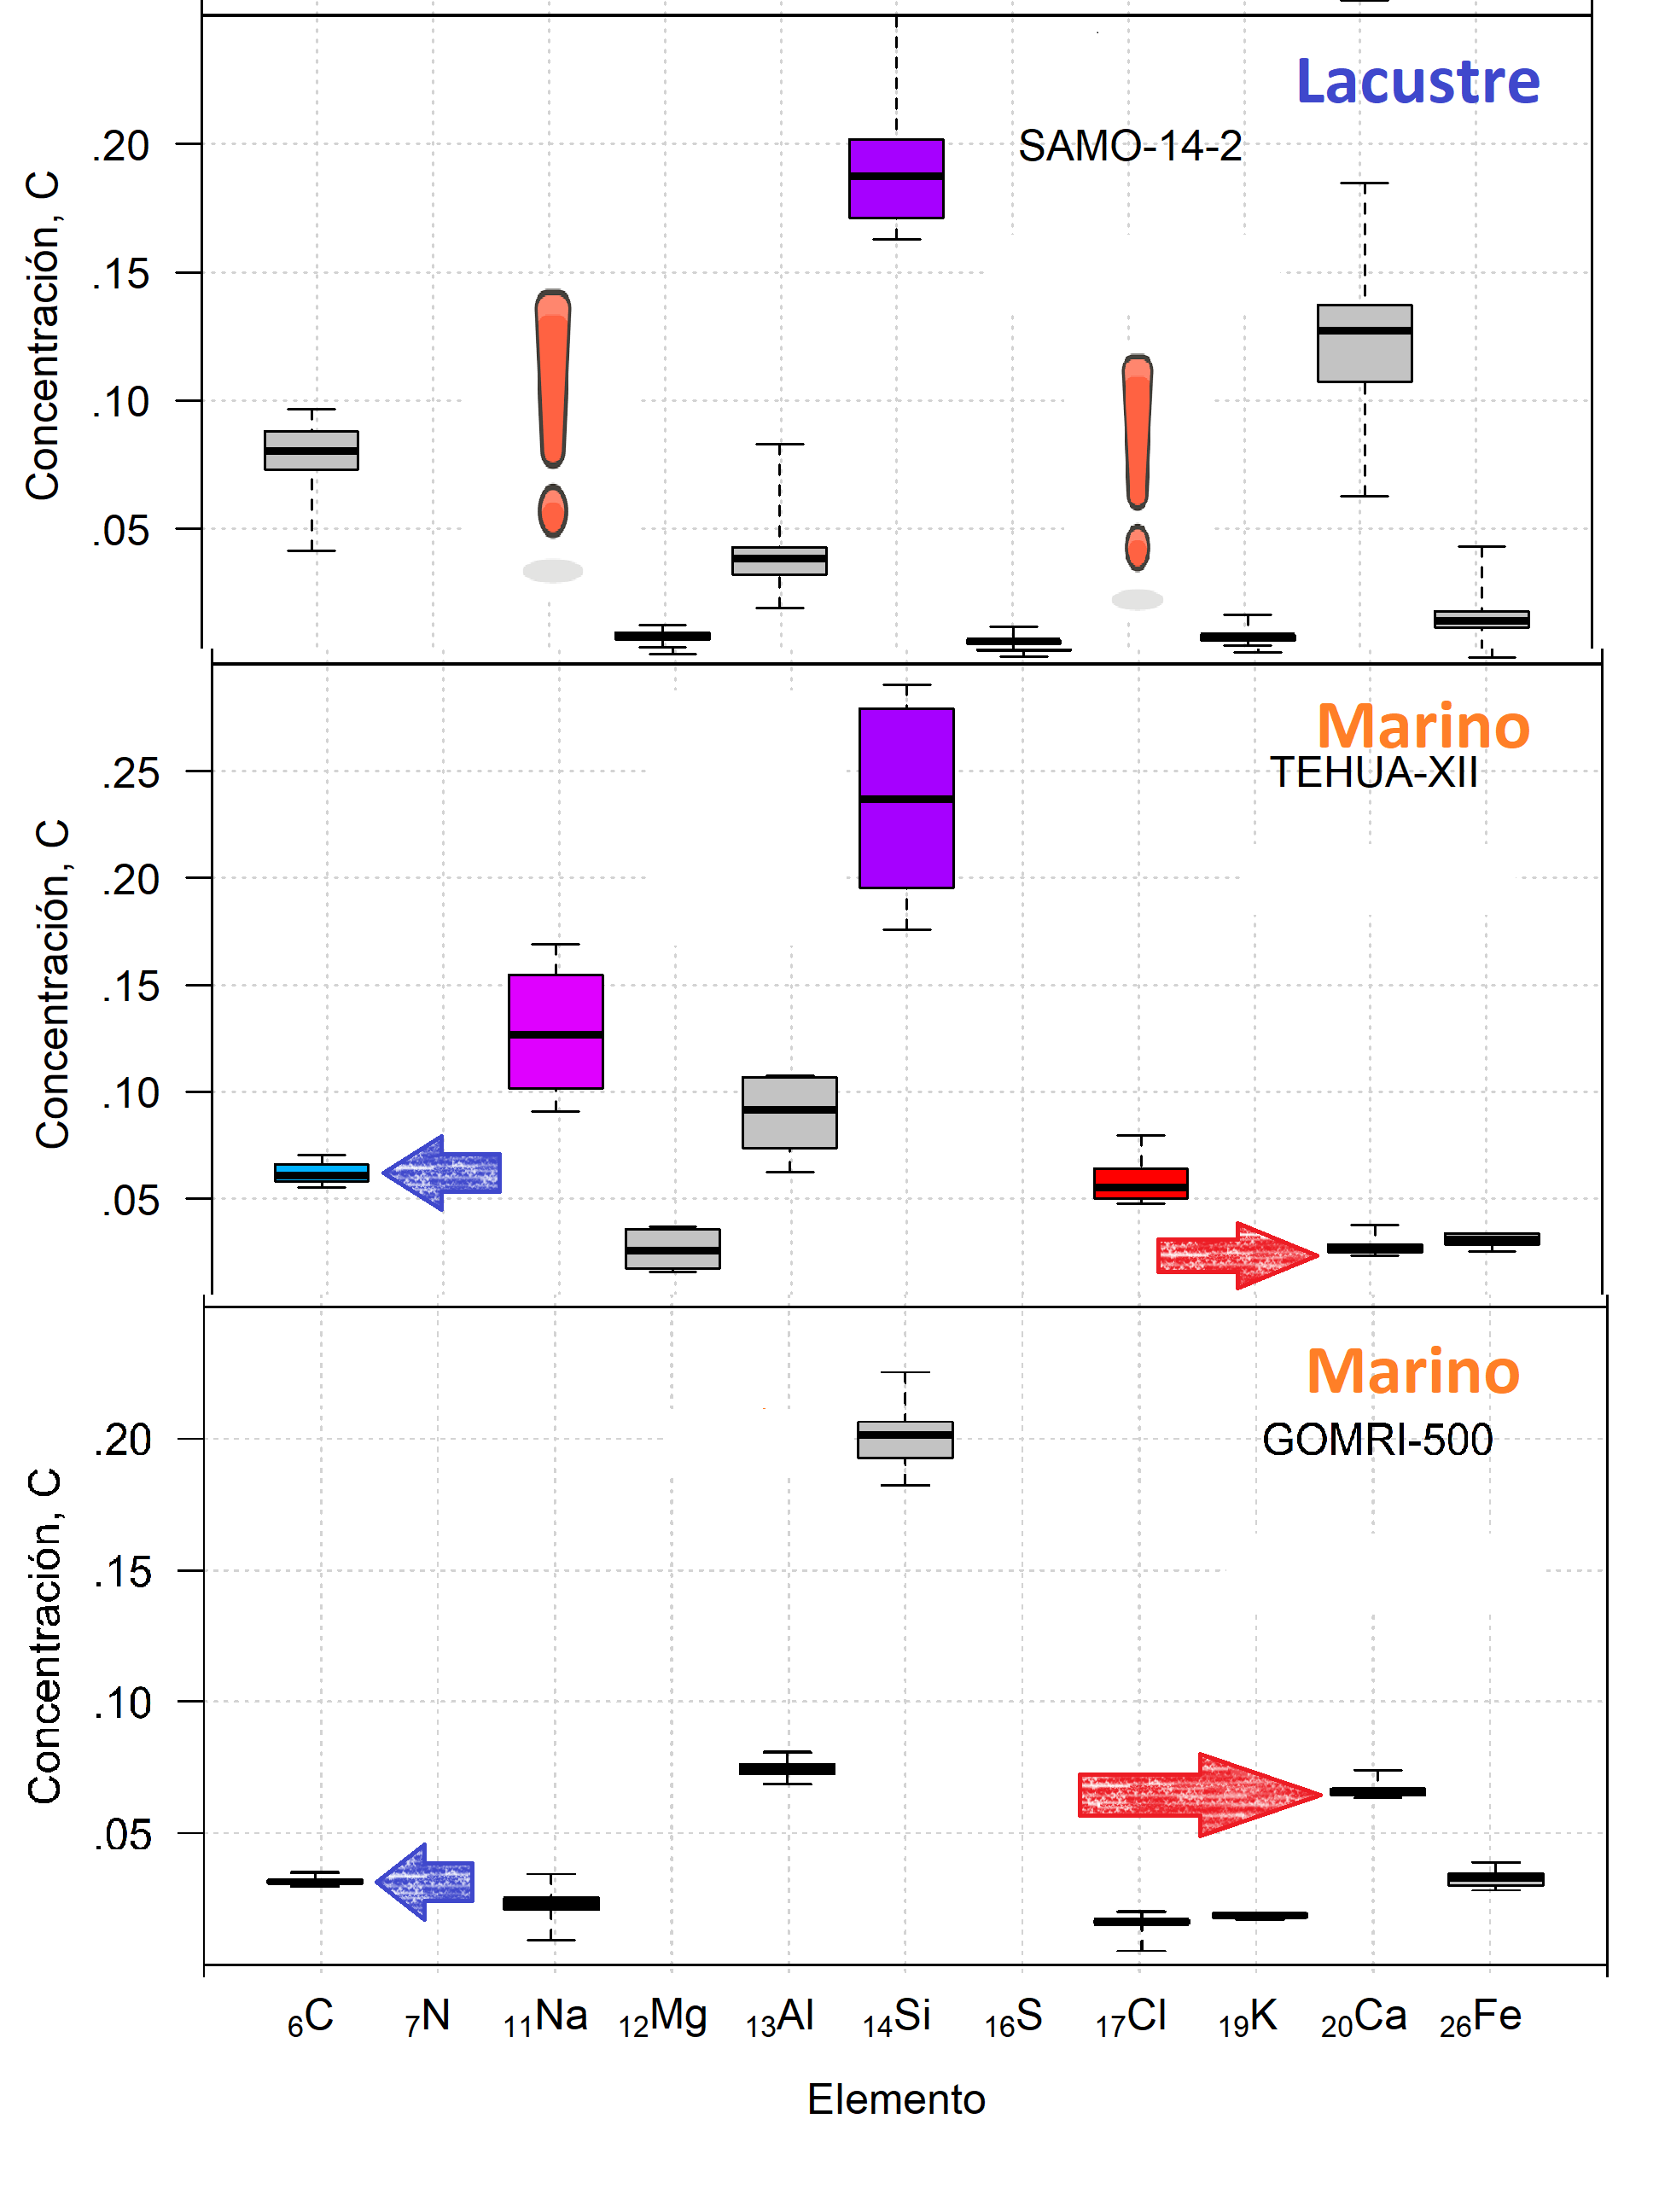
\includegraphics[width=0.48\textwidth]{Imagenes/XRF_Todos_Los_Nucleos_2-3.png}
	\end{figure}
\end{frame}

\begin{frame}{Composición elemental medida de los núcleos sedimentarios}
	\begin{figure}
	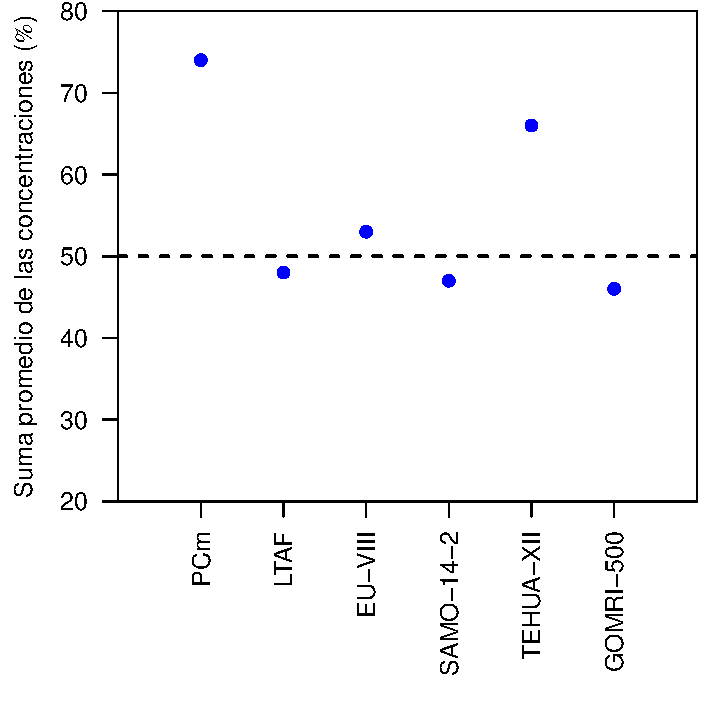
\includegraphics[width = 0.45\textwidth]{Imagenes/Resultados_Composicion.pdf}
	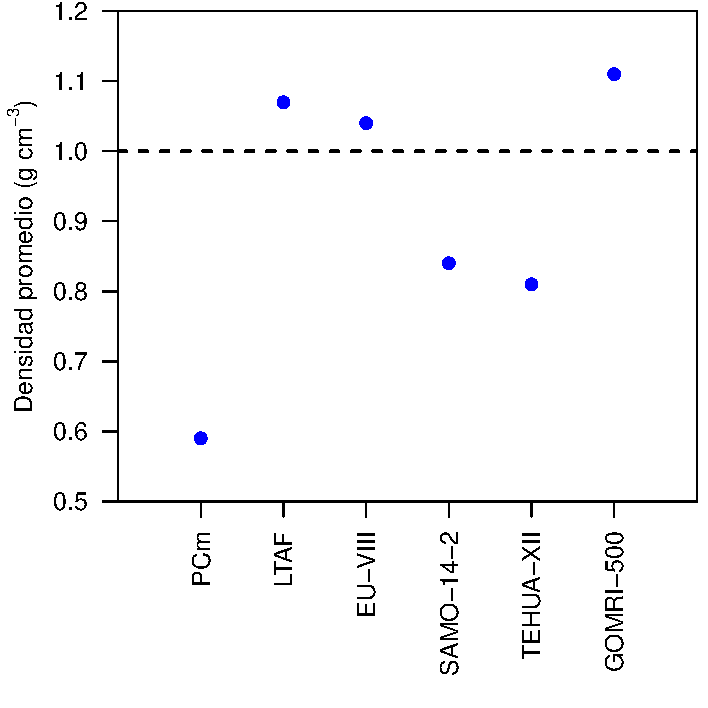
\includegraphics[width = 0.45\textwidth]{Imagenes/Resultados_Densidad.pdf}
	\caption{\justifying Suma de las concentraciones absolutas promedio medidas y valor de la densidad promedio $\overline{\rho}$ (en g cm$^{-3}$) a lo largo de los núcleos sedimentarios.}
	\end{figure}

\end{frame}

\begin{frame}{Composición corregida}
\begin{figure}
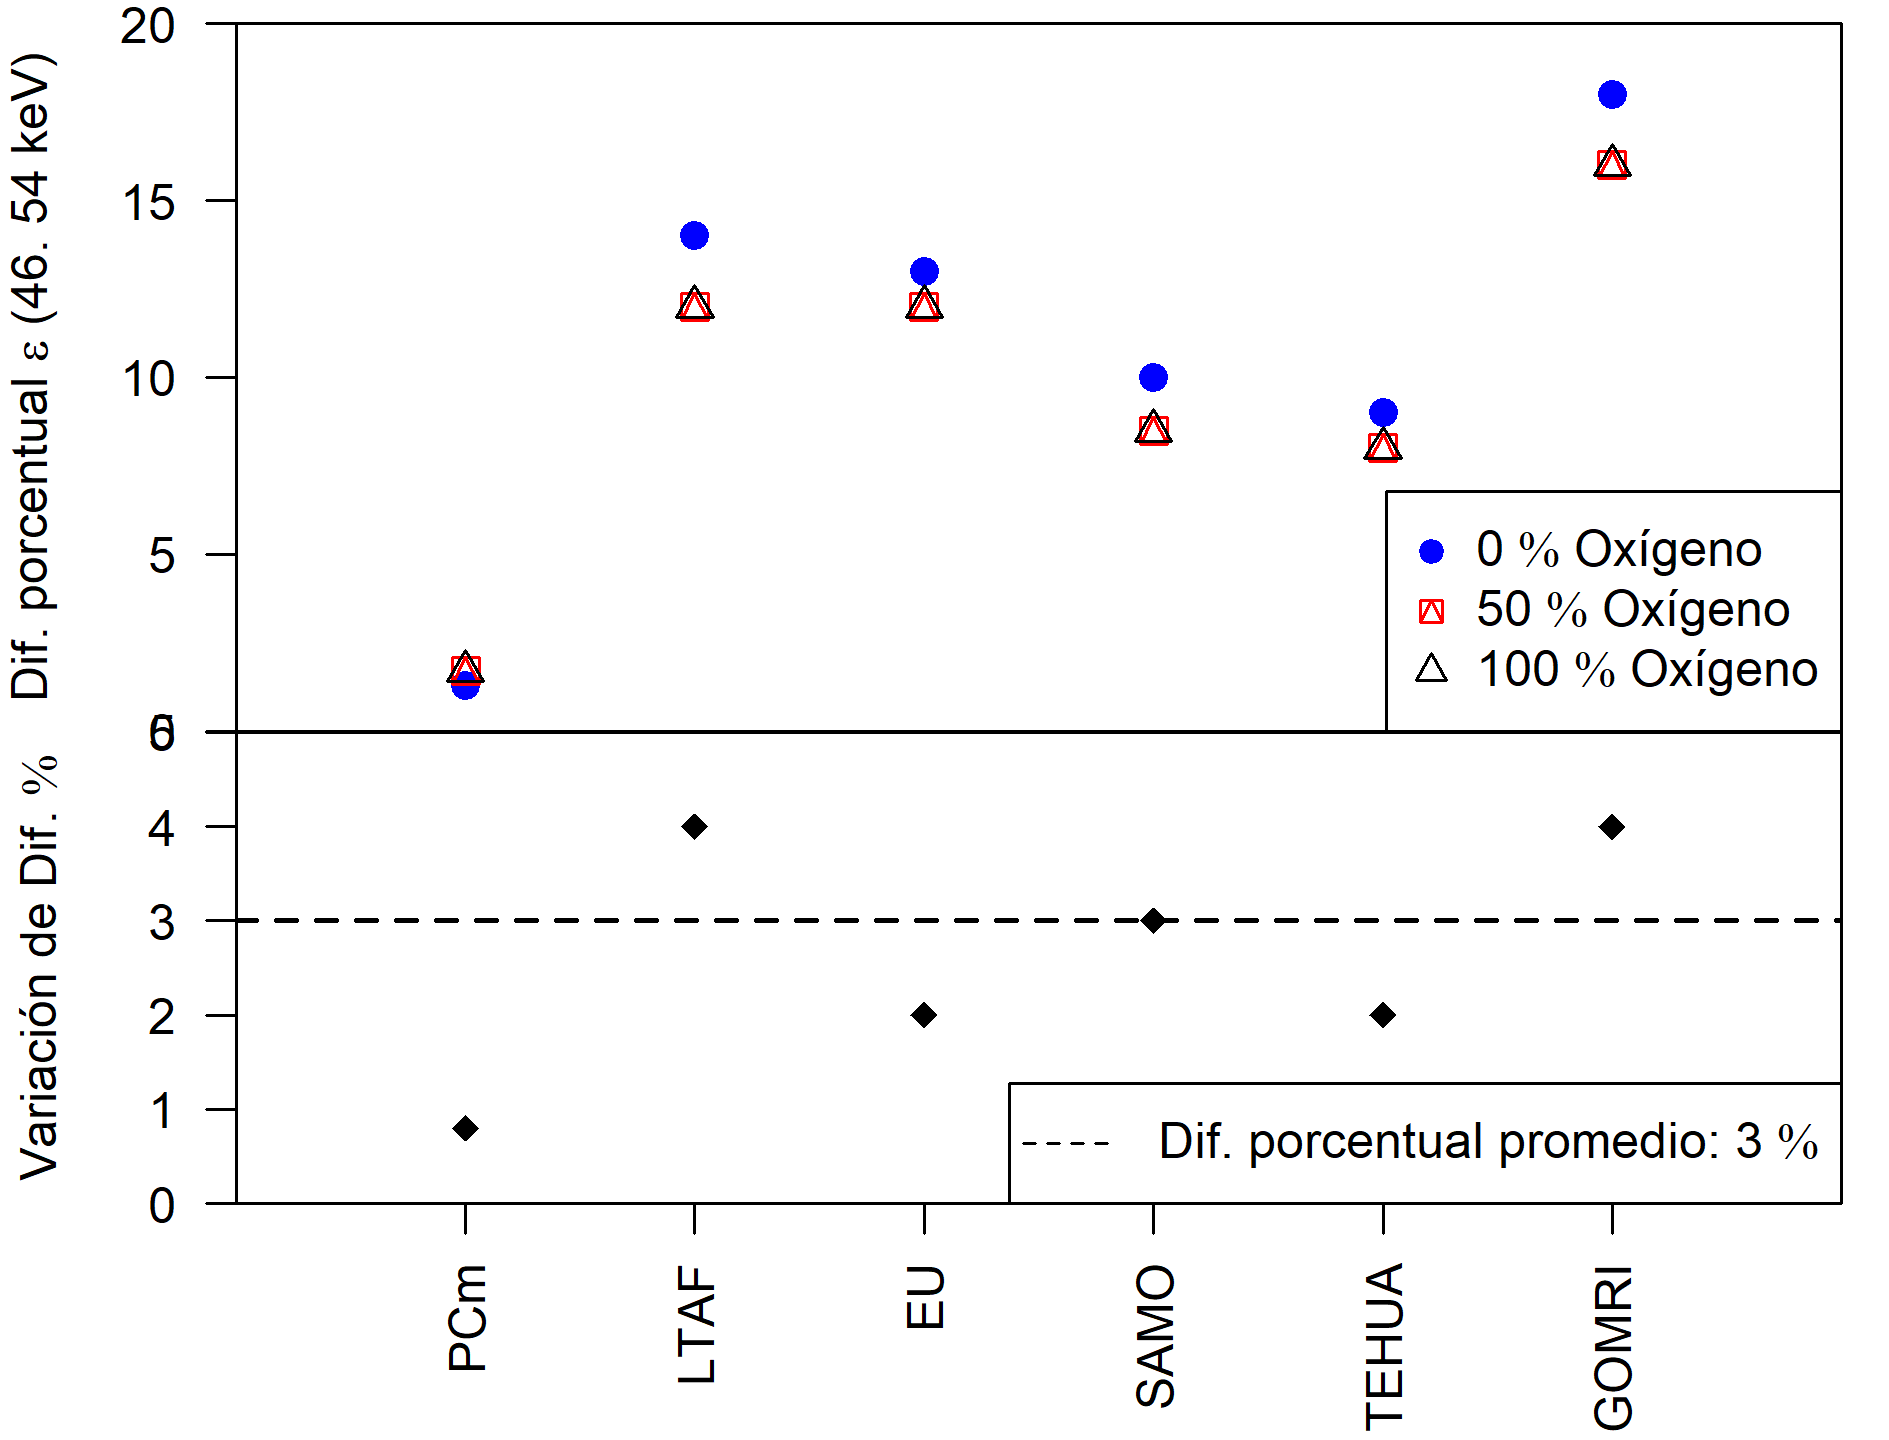
\includegraphics[width = 0.6\textwidth]{Imagenes/Resultados_DiffPorcentualEficiencia_FECHP_20190618.png}
\end{figure}

La desviación promedio calculada (3 \%) es inferior a la incertidumbre de la medida 
\begin{center}
\textbf{$\therefore$ composición corregida = 50 \% oxígeno y 50 \% hidrógeno de $X_\text{desconocido}$.}
\end{center}
\end{frame}

\begin{frame}{Perfiles de \PbCero\, para una composición de referencia y corregida}
	\begin{figure}
		\centering
		\includegraphics[width=0.45\textwidth]{Imagenes/Act_210Pb_Agua_Composicion_PCm.png}
		\includegraphics[width=0.45\textwidth]{Imagenes/Act_210Pb_Agua_Composicion_LTAF.png}
		\caption{ \textbf{PCm} y \textbf{LTAF} }
		\end{figure}
\end{frame}

\begin{frame}{Perfiles de \PbCero\, para una composición de referencia y corregida}
	\begin{figure}
		\centering
		\includegraphics[width=0.45\textwidth]{Imagenes/Act_210Pb_Agua_Composicion_EU_VIII.png}
		\includegraphics[width=0.45\textwidth]{Imagenes/Act_210Pb_Agua_Composicion_SAMO-14-2.png}
		\caption{\textbf{EU-VIII} y \textbf{SAMO-14-2} }

	\end{figure}
\end{frame}

\begin{frame}{Perfiles de \PbCero\, para una composición de referencia y corregida}
	\begin{figure}
		\centering
		\includegraphics[width=0.45\textwidth]{Imagenes/Act_210Pb_Agua_Composicion_TEHUA-XII.png}
		\includegraphics[width=0.45\textwidth]{Imagenes/Act_210Pb_Agua_Composicion_GOMRI_500.png}
		\caption{ \textbf{TEHUA-XII} y \textbf{GOMRI-500}}
	\end{figure}
\end{frame}

\begin{frame}{Perfiles de \PbCero\, para una composición de referencia y corregida}
	\begin{figure}
		\centering
		\includegraphics[width=0.45\textwidth]{Imagenes/Act_210Pb_Agua_Composicion_TEHUA-XII.png}
		\includegraphics[width=0.45\textwidth]{Imagenes/Act_210Pb_Agua_Composicion_GOMRI_500-2.png}
		\caption{ \textbf{TEHUA-XII} y \textbf{GOMRI-500}}
	\end{figure}
\end{frame}

\begin{frame}{Perfiles de \PbCero\, y \PbCuatro.}
	\begin{figure}
		\centering 
		\includegraphics[width=0.7\textwidth]{Imagenes/Graficas_Perfiles_Todos_20190509-2.png}
	\end{figure}
	\begin{flushleft}
\hyperlink{Diagenesis}{\beamerbutton{Diag}} \hyperlink{Shape}{\beamerbutton{Shape}}
\end{flushleft}
\end{frame}

\begin{frame}[noframenumbering]{Perfiles de \PbCero\, y \PbCuatro.}
	\begin{figure}
		\centering 
		\includegraphics[width=0.7\textwidth]{Imagenes/Graficas_Perfiles_Todos_20190509-3.png}
	\end{figure}
	\begin{flushleft}
\hyperlink{Diagenesis}{\beamerbutton{Diag}} \hyperlink{Shape}{\beamerbutton{Shape}}
\end{flushleft}
\end{frame}

\begin{frame}{Equilibrio secular}
			\begin{equation}
			\delta = \dfrac{A(^{214}\text{Pb}) - A(^{210}\text{Pb}) }{A(^{214}\text{Pb}) } \times 100
			\end{equation}
			\begin{figure}
				\centering
				\includegraphics[width=0.6\textwidth]{Imagenes/Grafica_Delta_210Pb_214Pb-3.png}
				\caption{\justifying Diferencia porcentual $\delta$ de los valores de la actividad específica de \PbCero\, respecto a la actividad específica de \PbCuatro\, para las secciones que se encuentran en equilibrio.}
			\end{figure}
\end{frame}

\begin{frame}{Modelos de edad para dos composiciones}
	\begin{figure}
		\centering
		\includegraphics[width=0.45\textwidth]{Imagenes/PCm_1.png}
		\includegraphics[width=0.45\textwidth]{Imagenes/LTAF_1.png}
		\caption{ \textbf{PCm} y \textbf{LTAF}}
	\end{figure}
\end{frame}

\begin{frame}{Modelos de edad para dos composiciones}
	\begin{figure}
		\centering
		\includegraphics[width=0.45\textwidth]{Imagenes/EUVIII_1.png}
				\includegraphics[width=0.45\textwidth]{Imagenes/SAMO142_1.png}

		\caption{ \textbf{EU-VIII} y \textbf{SAMO-14-2}}
	\end{figure}
\end{frame}

\begin{frame}{Modelos de edad para dos composiciones}
	\begin{figure}
		\centering
		\includegraphics[width=0.45\textwidth]{Imagenes/TEHUA_1.png}
		\includegraphics[width=0.45\textwidth]{Imagenes/GOMRI500_1.png}
		\caption{ \textbf{TEHUA-XII} y \textbf{GOMRI-500}}
	\end{figure}
\end{frame}

\begin{frame}{Diferencias porcentuales en modelos de edad}
\begin{figure}
\includegraphics[width=0.7\textwidth]{Imagenes/Resultados_Fechado.pdf}
\end{figure}
			\begin{equation}
t(i) = \dfrac{1}{\lambda}\,\ln\left(\dfrac{\sum_{j=1}^\infty A_j\, m_j}{ \sum_{j=i+1}^\infty A_j\, m_j}\right). 
			\end{equation}	
\end{frame}

\section{Conclusiones}

\begin{frame}{Conclusiones}
\begin{itemize}
\item \justifying  Se seleccionaron los núcleos sedimentarios: EU-VIII, GOMRI-500, PCm, LTAF, SAMO-14-2 y TEHUA-XII. Gran variabilidad en la composición elemental inter- e intra-núcleos, de los que se conoce 46 \% hasta 75 \% de su composición promedio. 

\item \justifying  Composición corregida: XRF + C-N + composición desconocida con el 50 \% de contribución de oxígeno y el 50 \% de hidrógeno. 

\item \justifying  La diferencia entre la eficiencia de todas las muestras varió entre 1.7 y 16 \%. 

\item \justifying  Las desviaciones de las actividades de \PbCero\, fueron de 10 \% para EU-VIII, LTAF, SAMO-14-2 y TEHUA-XII, y de 16 \% para GOMRI-500 para composiciones de referencia y corregidas. 

\item \justifying  PCm presentó el mayor porcentaje de composición conocida promedio (75 \%), una diferencia promedio de 1.7 \% entre las eficiencias y una diferencia próxima a cero entre los modelo de fechado. 

\item \justifying  Se realizó el fechado de los núcleos sedimentarios utilizando el modelo CF. Las fechas corregidas variaron entre 0.1 \% y 22 \%. Estas desviaciones no se correlacionaron de forma simple con la corrección de la eficiencia (y por lo tanto de la actividad) ni con su variabilidad, pues el modelo de edad incluye de forma compleja las sumas de los productos de las masas y las concentraciones. 
\end{itemize}
\begin{flushright}
\hyperlink{Portada}{\beamerbutton{Portada}}
\end{flushright}
\end{frame}
%\end{comment} 
\begin{frame}{Conclusión}
\justifying En la mayoría de los núcleos sedimentarios analizados se desconoce el 50 \% de su composición elemental. Esto puede causar una diferencia porcentual en el valor de las actividades de \PbCero\, de 16 \% y una diferencia de hasta 22 \% en el fechado, por lo tanto, es necesario siempre corregir la eficiencia, la actividad y el fechado debido a su composición. 
\begin{flushright}
\hyperlink{Portada}{\beamerbutton{Portada}}
\end{flushright}
\end{frame}

\begin{frame}[noframenumbering]
\begin{flushright}
\guillemotleft \textit{Así es} - suspiró el coronel -. \\ \vspace{0.2cm}
\textit{La vida es la cosa mejor que se ha inventado}. \guillemotright
\begin{footnotesize}
\\ \vspace{0.5cm}
Gabriel García Márquez
\\
El coronel no tiene quien le escriba, 1961.
\end{footnotesize}
\end{flushright}
\vspace{1cm}

\begin{flushright}
\hyperlink{Portada}{\beamerbutton{Portada}}
\end{flushright}
\end{frame}

%Titulo opcional de la tesis
\begin{frame}[noframenumbering, label=Portada2]{Título opcional para la tesis}
	\begin{center}
	\textbf{Corrección de las actividades y del fechado con \PbCero\, debido a la composición elemental para núcleos sedimentarios acuáticos mexicanos.}
	\end{center}
	\begin{flushright}
	\hyperlink{Portada}{\beamerbutton{Portada}}
	\end{flushright}
\end{frame}

% Equilibrio Secular
\begin{frame}[noframenumbering, label=EquilibrioSecular]{Equilibrio Secular}
En una serie de desintegración radiactiva, sea el núcleo progenitor $A$ y los núcleos radiactivos descendientes $B$ y $C$, y las condiciones iniciales
\begin{equation}
N_A(t=0) = N_{A,0}, \hspace{0.2cm} N_B(t=0) = N_C(t=0) = 0
\end{equation}
\begin{eqnarray}
N_A(t) &=& N_{A,0}\,\exp(-\lambda_A\,t) \\
N_B(t) &=& \dfrac{\lambda_A}{\lambda_B-\lambda_A}\,N_{A,0}\biggl[ \exp(-\lambda_A\,t) - \exp(-\lambda_B\,t) \biggr] \\
N_C(t) &=& \alpha\,\exp(-\lambda_A\,t) + \beta\,\exp(-\lambda_B\,t) + \gamma\,\exp(-\lambda_C\,t) \\
\alpha &=& \dfrac{\lambda_A\,\lambda_B}{(\lambda_C-\lambda_A)(\lambda_B-\lambda_A)}\,N_{A,0} \\
\beta &=& - \dfrac{\lambda_A\,\lambda_B}{(\lambda_C-\lambda_B)(\lambda_B-\lambda_A)} \,N_{A,0} \\
\gamma &=& -\lambda-\beta  
\end{eqnarray}
\begin{equation}
\text{Actividad}(t) = N(t)\,\lambda
\end{equation}
	\begin{flushright}
	\hyperlink{Portada}{\beamerbutton{Portada}}
	\end{flushright}
\end{frame}

\begin{frame}[noframenumbering]{Equilibrio Secular}
Para 
\begin{equation}
T_{\frac{1}{2}, A} = 1500, \hspace{1cm} T_{\frac{1}{2}, B} = 0.014, \hspace{1cm} T_{\frac{1}{2}, C} = 20,
\end{equation}
\begin{figure}
\includegraphics[height=0.4\textheight]{Imagenes/EquilibrioSecular1.png}
\includegraphics[height=0.4\textheight]{Imagenes/EquilibrioSecular2.png}
\end{figure}
\begin{equation}
\text{Actividad}(t) = N(t)\,\lambda
\end{equation}
	\begin{flushright}
	\hyperlink{Portada}{\beamerbutton{Portada}}
	\end{flushright}
\end{frame}

% Diagénesis 
\begin{frame}[noframenumbering, label=Shape]{Forma de los perfiles de \PbCero}
\begin{figure}
\includegraphics[width=0.8\textwidth]{Imagenes/Shape.png}
\end{figure}

	\begin{flushright}
	\hyperlink{Portada}{\beamerbutton{Portada}}
	\end{flushright}
\end{frame}

% Diagénesis 
\begin{frame}[noframenumbering, label=Diagenesis]{Diagénesis}
Diagénesis: son los cambios físicos (compactación), bioquímicos (descomposición de hojas) o biológicos (infauna) en un depósito sedimentario. 
\\
\PbCero\, en el sedimentario puede ser afectado por 
\begin{itemize}
\item Presencia de aniones Cl$^{-}$, HCO$_3^{-}$, SO$_4^{-2}$
\item Oxidación de $^{210}$PbS
\item Formación de sulfuros insolubles
\item Aumento de SAR implica la descomposición de Materia Orgánica. Sediment Rate Acumulation, SAR, $\dfrac{\text{m}}{\text{año}}$, para lagos $>$ 1 cm/año y para mar $>$ 0.1 cm/año. 
\end{itemize}
	\begin{flushright}
	\hyperlink{Portada}{\beamerbutton{Portada}}
	\end{flushright}
\end{frame}

\begin{frame}[noframenumbering]{LTAF}
\justifying Un comportamiento inverso fue observado en el núcleo LTAF, pues las actividades de \PbCero\, son en este caso inferiores al \PbCuatro, lo que significa la presencia de un déficit de \PbCero, probablemente  debido a un enriquecimiento de \Ra\, (en equilibrio con el \PbCuatro) debido a procesos diagenéticos. De hecho, LTAF es el núcleo sedimentario de manglar con mayor concentración de \PbCero, que puede ser debido a la migración hacia la superficie de \Ra<  \, de capas inferiores, causando así su exceso respecto al \PbCero. Esto es consistente con el decrecimiento del \PbCuatro\, en las capas superficiales, indicando que parte del \Ra\, está siendo transferido al agua intersticial, y de aquí a la columna de agua. En estos casos, es recomendable utilizar las concentraciones de \PbCero\, en el fondo del núcleo para estimar un valor constante del \PbCeroEx. 
	\begin{flushright}
	\hyperlink{Portada}{\beamerbutton{Portada}}
	\end{flushright}
\end{frame}

% Fechado 
\begin{frame}[noframenumbering, label=Fechado]{Fechado}
\begin{itemize}
\item Es un modelo.
\item Capas (ayuda matemática, $(i)$) y secciones (¡existe!, tiene masa, concentración de \PbCero, $_i$ ).
\item Sedimento: ¿Cuánto sedimento (metros) cae por unidad de tiempo (año)? SAR, $s$, y, para 1 metro$^2$, ¿cuánto sedimento (kg) pasa en un año? MAR, $r = \dfrac{dm}{S\,dt}$.
\item $f$ es el flujo de \PbCero. 
\end{itemize}
 \begin{equation}
r = \rho\,s.
\end{equation}
\begin{equation}
A(i,t=0) = \dfrac{f(i)}{r(i)} \hspace{0.5cm}
\rightarrow \hspace{0.5cm} A(i)	= \dfrac{f}{r(i)}\,\exp(-\lambda\,t) 
\end{equation}
\begin{equation}
\mathbb{A}(i) = \sum_{j=i+1}^{j\rightarrow \infty} \bigtriangleup \mathbb{A}_j = \int_m^\infty A\, dm =  
\int_m^\infty \dfrac{f}{r}\,\exp(-\lambda\,t)\, dm =  \dfrac{f}{\lambda}\,\exp(-\lambda\,t).
\end{equation}
\begin{equation}
\mathbb{A}(i) = \mathbb{A}(0)\,\exp(-\lambda\,t).
\end{equation}
\begin{equation}\label{Eq-Fechado}
t(i) = \dfrac{1}{\lambda}\,\ln\left(\dfrac{\mathbb{A}(0)}{\mathbb{A}(i)}\right) = \dfrac{1}{\lambda}\,\ln\left(\dfrac{\sum_{j=1}^\infty A_j\, m_j}{ \sum_{j=i+1}^\infty A_j\, m_j}\right)
\end{equation}

	\begin{flushright}
	\hyperlink{Portada}{\beamerbutton{Portada}}
	\end{flushright}
\end{frame}

% Coeficiente másico de atenuación
\begin{frame}[noframenumbering, label=Masico]{Coeficiente másico de atenuación}
		 Ley de atenuación exponencial$^{1,2}$
		\begin{equation}
			\dfrac{I}{I_0} = \exp\left[-\dfrac{\mu}{\rho}\,\rho\,x\right], \hspace{0.5cm} \dfrac{\mu}{\rho} = \dfrac{\sigma_\text{total}}{u\,A},
		\end{equation}
		donde $u$ es la unidad de masa atómica y $A$ el número de nucleones.
	\begin{flushright}
	\hyperlink{Portada}{\beamerbutton{Portada}}
	\end{flushright}
\end{frame}

%Sección eficaz
\begin{frame}[noframenumbering, label=SeccionEficaz]{Sección eficaz}
\begin{eqnarray}
\sigma &=& \dfrac{\text{Número de reacciones por blanco por segundo}}{\text{Flujo de proyectiles}} \\
\sigma&=& \dfrac{\dfrac{\text{No. de reacciones}}{\text{segundo}}}{\dfrac{\text{No. de proyectiles}}{\text{área}\times\text{segundo}}} \\
\sigma&=& \text{área} \hspace{1cm} \rightarrow \hspace{1cm} \text{1 barn = }10^{-24} \text{cm}^2
\end{eqnarray}

\begin{equation}
\sigma_{\text{foto}} \propto  
  \begin{cases}
    Z^5\, E^{-3.5},	& 13.6 \text{ eV} < E<m_e\,c^2, \\
    Z^5\, E^{-1},	& E > m_e\,c^2.
  \end{cases}
\end{equation}

\begin{equation}
\sigma_\text{Comp} \propto
  \begin{cases}
    \sigma_{\text{Thompson}}(1-2\,\epsilon),	& E \ll m_e\,c^2, \\
    \log(\epsilon)\, \epsilon^{-1} \,Z,		&  E \gg m_e\,c^2,
  \end{cases}
\end{equation}
donde $\epsilon = \dfrac{E}{m_e\,c^2}$ y $\sigma_{\text{Thompson}}$ = 0.66 barn.
	\begin{flushright}
	\hyperlink{Portada}{\beamerbutton{Portada}}
	\end{flushright}
\end{frame}

\begin{frame}[noframenumbering, label=SeccionEficaz]{Sección eficaz}
\begin{figure}
\includegraphics[width=0.4\textwidth]{Imagenes/FeymannPhotoelectric.png}
\includegraphics[width=0.4\textwidth]{Imagenes/FeymannCompton.png}
\end{figure}
	\begin{flushright}
	\hyperlink{Portada}{\beamerbutton{Portada}}
	\end{flushright}
\end{frame}

% TCSC
\begin{frame}[noframenumbering, label=TCSC]{TCSC - True Coincidence Summing Correction}
\justifying True coincidence summing (TCS) occurs when two or more photons are emitted from the same decay of a radioactive nuclide and are detected within the resolving time of the gamma ray detector.
\begin{figure}
\includegraphics[width=0.6\textwidth]{Imagenes/134Cs.png}
\end{figure}
	\begin{flushright}
	\hyperlink{Portada}{\beamerbutton{Portada}}
	\end{flushright}
\end{frame}

%Espectros 
\begin{frame}[noframenumbering, label=Espectros]{Espectros: información general}
\begin{figure}
\includegraphics[width=0.7\textwidth]{Imagenes/Espectro.png}
\end{figure}
	\begin{flushright}
	\hyperlink{Portada}{\beamerbutton{Portada}}
	\end{flushright}
\end{frame}

\begin{frame}[noframenumbering]{Espectros: información general}
\begin{figure}
\includegraphics[width=0.7\textwidth]{Imagenes/SingleDoubleEscape.png}
\end{figure}
	\begin{flushright}
	\hyperlink{Portada}{\beamerbutton{Portada}}
	\end{flushright}
\end{frame}

\begin{frame}[noframenumbering]{Espectro de TEHUA-XII}
\begin{figure}
\includegraphics[width=0.9\textwidth]{Imagenes/EspectroTEHUA.png}
\end{figure}
	\begin{flushright}
	\hyperlink{Portada}{\beamerbutton{Portada}}
	\end{flushright}
\end{frame}

\begin{frame}[noframenumbering]{Espectro de TEHUA-XII, \PbCero\, y \PbCuatro}
\begin{figure}
\includegraphics[width=0.45\textwidth]{Imagenes/EspectroTEHUAPb210.png}
\includegraphics[width=0.45\textwidth]{Imagenes/EspectroTEHUAPb214.png}
\end{figure}
	\begin{flushright}
	\hyperlink{Portada}{\beamerbutton{Portada}}
	\end{flushright}
\end{frame}

\begin{frame}[noframenumbering]{Espectro de fondos}
\begin{figure}
\includegraphics[width=0.75\textwidth]{Imagenes/Fondos.pdf}
\end{figure}
	\begin{flushright}
	\hyperlink{Portada}{\beamerbutton{Portada}}
	\end{flushright}
\end{frame}

% Tiempo muerto
\begin{frame}[noframenumbering]{Tiempo muerto}
\begin{figure}
\includegraphics[width=0.95\textwidth]{Imagenes/TiempoMuerto.png}
\end{figure}
	\begin{flushright}
	\hyperlink{Portada}{\beamerbutton{Portada}}
	\end{flushright}
\end{frame}

%RPT
\begin{frame}[noframenumbering]{Archivo RPT de EU-VIII 21.5 cm}
\begin{figure}
\includegraphics[width=0.5\textwidth]{Imagenes/InformationEUVIII.png}
\end{figure}
	\begin{flushright}
	\hyperlink{Portada}{\beamerbutton{Portada}}
	\end{flushright}
\end{frame}


\begin{frame}[noframenumbering, label=Ciclo]{El ciclo de \PbCero\, en ecosistemas acuáticos}
La actividad de \PbCero\, presente en los sedimentos puede tener diversos orígenes:
\begin{itemize}
\justifying
\item La desintegración de \Rn, núcleo precursor de \PbCero, que es un gas noble y puede escapar de la tierra hacia la atmósfera después de la desintegración del núcleo progenitor \Ra. \Rn\, decae en la atmósfera en una corta serie de núcleos de vida media corta ($\sim$ minutos) hasta \PbCero. Debido a la alta reactividad del Pb con las partículas, el \PbCero\, se une a partículas en suspensión y sedimenta al fondo de los sistemas acuáticos.  
\item \Rn\, puede escapar de la litosfera directamente a los cuerpos de agua y decaer en \PbCero, que también sedimenta al fondo. La suma de este componente y la anterior se denomina \PbCero\, en exceso, \PbCeroEx, que es la base del fechado de sedimentos con \PbCero.
\item \Rn\, que no escapa sino que se desintegra \textit{in situ} y decae en \PbCero, conocido como $^{210}$Pb$_\text{base}$. Para sistemas cerrados por tiempos superiores a 150 años, $^{210}$Pb$_\text{base}$ se encuentra en equilibrio con el radionúclido \Ra\, con $T_{\frac{1}{2}}$ (\Ra) = 1600(7) años. 
\end{itemize}
	\begin{flushright}
	\hyperlink{Portada}{\beamerbutton{Portada}}
	\end{flushright}
\end{frame}


% \item Características núcleos sedimentarios, espectrometría alfa y gamma
% \item Detectores de Ge. 

\end{document}
